\documentclass[12pt, oneside]{ThesisKazmi} % The default font size and one-sided printing (no margin offsets)
\graphicspath{{Pictures/}}
\usepackage{hyperref}
%\usepackage[style=ieee]{biblatex}
\usepackage[square, numbers, comma, sort&compress]{natbib}
\hypersetup{urlcolor=blue, colorlinks=true}
\usepackage{setspace}
\usepackage{fancyhdr, graphicx}
\usepackage{lscape}
\usepackage[noadjust]{cite}
\makeindex
\usepackage{makeidx}
\title{\ttitle}

 \begin{document}

\frontmatter % Use roman page numbering style (i, ii, iii, iv...) for the pre-content pages

\setstretch{1.3} % Line spacing of 1.3

% Define the page headers using the FancyHdr package and set up for one-sided printing
\fancyhead{} % Clears all page headers and footers
\rhead{\thepage} % Sets the right side header to show the page number
\lhead{} % Clears the left side page header

\pagestyle{fancy} % Finally, use the "fancy" page style to implement the FancyHdr headers

\newcommand{\HRule}{\rule{\linewidth}{0.5mm}} % New command to make the lines in the title page

 %PDF meta-data
\hypersetup{pdftitle={\ttitle}}
\hypersetup{pdfsubject=\subjectname}
\hypersetup{pdfauthor=\authornames}
\hypersetup{pdfkeywords=\keywordnames}

%----------------------------------------------------------------------------------------
%	TITLE PAGE
%----------------------------------------------------------------------------------------

\begin{titlepage}
\begin{center}
\textsc{\Large \textbf{Track A Shop: Web App}}\\[1.5cm] % University name
\begin{center}
\includegraphics[width=5.5cm]{Gculogo}\vspace{1cm}\\  % University/department logo - uncomment to place it
\end{center}
\large
\begin{center}
\textbf{\begin{tabular}{ p{5cm}   p{7cm} }
  % after \\: \hline or \cline{col1-col2} \cline{col3-col4} ...
  Submitted by & Muhammad Zeeshan Yousaf \\
  & Fatima Yousaf \\ [1ex]
  Roll. No & 0259-BSCS-19 \\
  & 0279-R-BSCS-19\\ [1ex]
  Session & 2019 - 2023 \\ [1ex]
  Supervised by & Sir Yahya Khurram \\
   & Assistant Professor\\
\end{tabular}}
\end{center}
%\begin{quote}
%\end{quote}

\vspace{1.5cm}
\large \textbf{BS(HONS)\\ IN \\ COMPUTER SCIENCE}\\
\vspace{1cm}
\textbf{\Large DEPARTMENT OF COMPUTER SCIENCE}\\ [0.3cm]% Thesis title
\textbf{{\Large GC UNIVERSITY LAHORE}}\\ % Research group name and department name
\vfill
\end{center}
\end{titlepage}
\begin{titlepage}
\begin{center}
\textsc{\Large \textbf{Track A Shop: Web App}}\\[1.5cm] % University name
%\begin{center}
%\includegraphics[width=5.5cm]{Gculogo}\vspace{1cm}\\  % University/department logo - uncomment to place it
%\end{center}
\large
\begin{center}
\textbf{Submitted to GC University Lahore
in partial fulfillment of the requirements
for the award of degree of}\\
\vspace{1.7cm}
\Large \textbf{BS(HONS)\\ IN \\ COMPUTER SCIENCE}\\
\vspace{2cm}
\large

\textbf{\begin{tabular}{ p{5cm}   p{7cm} }
  % after \\: \hline or \cline{col1-col2} \cline{col3-col4} ...
  Submitted by & Muhammad Zeeshan Yousaf \\
  & Fatima Yousaf \\ [1ex]
  Roll. No & 0259-BSCS-19 \\
  & 0279-R-BSCS-19 \\ [1ex]
  Session & 2019 - 2023 \\ [1ex]
  Supervised by & Sir Yahya Khurram\\
   & Assistant Professor\\
\end{tabular}}
\end{center}
%\begin{quote}
%\end{quote}
\vspace{4cm}
\textbf{\Large DEPARTMENT OF COMPUTER SCIENCE}\\ [0.5cm]% Thesis title
\textbf{{\Large GC UNIVERSITY LAHORE}} % Research group name and department name
%
%{\large \today}\\[2cm] % Date


\vfill
\end{center}
\end{titlepage}

\setstretch{1.5} % Reset the line-spacing to 1.5 for body text (if it has changed)
\clearpage % Start a new page

\Declaration{

\addtocontents{toc}{\vspace{1em}} % Add a gap in the Contents, for aesthetics

We, Muhammad Zeeshan Yousaf and Fatima Yousaf students of \textbf{BS (Hons)} in the subject of \textbf{Computer Science}\index{Computer Science}, session \textbf{2019-2023}, hereby declare that the material printed in this thesis titled, \textbf{Track A Shop: Web App} is our own work and has not been printed, published, or submitted as research work, thesis, or publication in any form in any university, research institution etc in Pakistan or abroad.\\
\vspace{2cm}

\textbf{Date: \line(1,0){100}} \hspace{100pt} \textbf{Signatures of Deponent}
}
\newpage
\flushbottom
\researchcompletioncertificate{\addtocontents{toc}{\vspace{1em}} % Add a gap in the Contents, for aesthetics

It is certified that the research work contained in this thesis titled \textbf{Track A Shop: Web App} has been carried out by \textbf{Muhammad Zeeshan Yousaf} Roll. No \textbf{0259-BSCS-19} and \textbf{Fatima Yousaf} Roll. No \textbf{0279-R-BSCS-19} under my supervision. \\
\vspace{2cm}\\
\large
\setstretch{1.0}
\begin{tabular}{p{5.5cm}   p{8.5cm}}
  % after \\: \hline or \cline{col1-col2} \cline{col3-col4} ...
  &\line(1,0){130}\\
   & \textbf{Sir Yahya Khurram} \\
   & \textbf{Assistant Professor}\\
   %& Department of Computer Science \\
%   & GC University Lahore
\end{tabular}

\vspace{50pt}

\textbf{Date: \line(1,0){90}} \\
\vspace{1.3cm}\\
\textbf{\textsc{Submitted Through}}\\
\vspace{4cm}\\

\setstretch{1.0}
\begin{tabular}{p{9.5cm}   p{7cm}}
  % after \\: \hline or \cline{col1-col2} \cline{col3-col4} ...
   \line(1,0){130} & \line(1,0){130} \\
   \textbf{Prof. Dr. Muhammad Waqas Anwar}  & \textbf{Controller of Examination}\\
   \textbf{Chairperson}  & \textbf{GC University Lahore} \\
\textbf{Department of Computer Science} &\\
\textbf{GC University Lahore} &\\
\end{tabular}

}

\clearpage % Start a new page

%----------------------------------------------------------------------------------------
%	ACKNOWLEDGEMENTS
%----------------------------------------------------------------------------------------

\setstretch{1.5} % Reset the line-spacing to 1.3 for body text (if it has changed)

\acknowledgements{\addtocontents{toc}{\vspace{1em}} % Add a gap in the Contents, for aesthetics
We are grateful to the Almighty Allah, Who blessed us with health, wisdom, knowledge, thoughts and opportunity to make some contribution in the form of present effort. We offer our humblest thanks from the deepest core of our heart to the \textbf{Holy Prophet Muhammad (Peace be upon him)}, the most perfect and excelled among and ever born on the surface of earth. The research work embodied in this dissertation was accomplished under the able guidance and affectionate supervision of \textbf{Sir Yahya Khurram}, GC University, Lahore. We will always remember his moral encouragement, skillful guidance, positive criticism and valuable advice throughout the course of our study. We also express our feelings of love and respect for our beloved parents that are the real asset of our life and gave us confidence.
%I am grateful to the Almighty \textbf{Allah}, Who blessed me with health, wisdom, knowledge, thoughts and opportunity to make some contribution in the form of present effort. I offer my humblest thanks from the deepest core of my heart to the \textbf{Holy Prophet Muhammad (Peace be upon him)}, the most perfect and excelled among and ever born on the surface of earth. \\
%The research work embodied in this dissertation was accomplished under the able guidance and affectionate supervision of \textbf{Dr. Muhammad Waqas Anwar}, Assistant Professor, GC University, Lahore. I will always remember his moral encouragement, skillful guidance, positive criticism and valuable advice throughout the course of my study. \\
%I also express my feelings of love and respect for my beloved parents that are the real asset of my life and gave me confidence and my friends also deserve my thanks for their loving encouragement and prayers for my success.

}
\clearpage % Start a new page


%----------------------------------------------------------------------------------------
%	DEDICATION
%----------------------------------------------------------------------------------------

\setstretch{1.5} % Return the line spacing back to 1.5

\pagestyle{empty} % Page style needs to be empty for this page
\dedication{
	\begin{center}
		\LARGE \textbf{Dedication} \\ [1cm]
		\large
		This project is dedicated to our family and our mentors, especially
		to our esteemed guide and teacher, for this project, who encouraged
		and supported us throughout the development and completion of
		"Track A Shop: Web App" - a leap in the realm of technology and
		innovation in computer science.
	\end{center}
} % Dedication text





\addtocontents{toc}{\vspace{2em}} % Add a gap in the Contents, for aesthetics



%----------------------------------------------------------------------------------------
%	ABSTRACT PAGE
%----------------------------------------------------------------------------------------

\addtotoc{Abstract} % Add the "Abstract" page entry to the Contents

\abstract{\addtocontents{toc}{\vspace{1em}} % Add a gap in the Contents, for aesthetics

\textbf{The "Track A Shop: Web App" project aims to address a significant issue prevalent in the digital era, where small businesses such as service providers, mini stores, and repair shops struggle to establish an online presence due to cost constraints. In response to this, we propose the development of a Web Application Software that acts as a centralized platform for local businesses to connect with their local customer base. By leveraging this application, shopkeepers can extend their reach and increase their earnings by reaching more customers online. Customers, in turn, can easily access and purchase products or avail services from nearby local shops within their specified geographical proximity. The project integrates an image recognition service, allowing sellers to effortlessly add products or services by simply uploading images. On the customer side, this service facilitates image-based search, enhancing the user experience and streamlining the purchasing process.}
	
\vspace{200pt}
\clearpage % Start a new page


%----------------------------------------------------------------------------------------
%	LIST OF CONTENTS/FIGURES/TABLES PAGES
%----------------------------------------------------------------------------------------

\pagestyle{fancy} % The page style headers have been "empty" all this time, now use the "fancy" headers as defined before to bring them back

\lhead{\emph{Contents}} % Set the left side page header to "Contents"
\tableofcontents % Write out the Table of Contents
\lhead{\emph{List of Tables}} % Set the left side page header to "List of Tables"
\listoftables % Write out the List of Tables
\lhead{\emph{List of Figures}} % Set the left side page header to "List of Figures"
\listoffigures % Write out the List of Figures


%----------------------------------------------------------------------------------------
%	ABBREVIATIONS
%----------------------------------------------------------------------------------------


%----------------------------------------------------------------------------------------
%	THESIS CONTENT - CHAPTERS
%----------------------------------------------------------------------------------------

\mainmatter % Begin numeric (1,2,3...) page numbering

\pagestyle{fancy} % Return the page headers back to the "fancy" style

% Include the chapters of the thesis as separate files from the Chapters folder
% Uncomment the lines as you write the chapters

% Chapter 1

\chapter{Introduction} % Main chapter title

\label{Chapter1} % For referencing the chapter elsewhere, use \ref{Chapter1}

\lhead{Chapter 1. \emph{Introduction}} % This is for the header on each page - perhaps a shortened title

%----------------------------------------------------------------------------------------

\section{Introduction}
In an era characterized by rapid technological advancements, businesses are constantly seeking efficient, automated, and precise solutions to streamline their operations. This paradigm shift has led to the creation of numerous software programs tailored to meet the diverse needs of different industries, facilities, and various workplaces. Historically, manual methods were employed for data management, but evolving preferences have spurred a transition to digital solutions. Recognizing the digital divide prevalent among small businesses, particularly those serving local communities, this project, "Track A Shop: Web App," endeavors to empower these enterprises and enable their seamless integration into the online marketplace.

In today's digital landscape, the majority of businesses across sectors have embraced online platforms to market and sell their products and services, swiftly reaching customers through home deliveries. However, smaller businesses such as service providers, mini stores, repair shops, and local vendors, including cobblers, barbers, milk shops, bakeries, and spare parts shops, often find it financially challenging to establish an online presence. The "Track A Shop: Web App" web application sets out to address this disparity by providing local shops a centralized online platform to connect with their local customer base. Through this application, shopkeepers can significantly broaden their customer reach, attract a larger audience, and consequently, enhance their earnings with minimal effort of input.

The project envisions simplifying and modernizing operations for local businesses by integrating innovative features such as image recognition for effortless addition of products services, and image-based search capabilities for customers.

\vspace{0.5cm}
\section{Project Overview}

The proposed system, "Track A Shop: Web App," is a web-based application designed to facilitate the seamless creation of online shops for sellers. Utilizing image recognition technology, sellers can effortlessly add products or services to their online shop by capturing or uploading images. The system automatically identifies and categorizes the items, making them readily accessible to customers in the vicinity of the shop. Conversely, customers can easily browse and search for products or services using images, names, or proximity filters. They can initiate requests for product delivery or obtain directions to the seller's physical shop, enhancing their overall shopping experience.

\vspace{0.5cm}
\section{Problem Statement}
In the contemporary business landscape, small enterprises encounter a significant barrier in establishing an online platform for their operations due to prohibitive costs associated with web development and maintenance. The high financial investment required often restricts their ability to tap into the potential of the digital marketplace, limiting their growth and outreach.

Furthermore, the traditional method of manually inputting products and services into an online platform has become increasingly burdensome and time-consuming. This arduous process not only consumes valuable time but also poses a hindrance to the efficient management and scaling of businesses, leading to decreased productivity and suboptimal user experiences.

In addition, both customers and local shops face challenges in connecting efficiently. The conventional approach of physically visiting or relying on word-of-mouth recommendations to discover shops or services is cumbersome and time-intensive. This lack of a seamless and convenient means to connect customers with local shops impedes the potential for increased business transactions and growth for these small enterprises. Therefore, an effective solution is imperative to address these pressing issues and bridge the existing gap between small businesses and their online presence while enhancing accessibility and connectivity for both customers and shops.

\vspace{0.5cm}
\section{Project Scope}
The scope of "Track A Shop: Web App" project encompasses the development of a comprehensive web-based platform targeting small businesses and local shops to establish an online presence for their products and services. The platform will facilitate seamless integration and accessibility for both sellers and customers. It will incorporate image recognition technology, allowing sellers to effortlessly list their products and services by capturing or uploading images. Customers can easily search for and purchase products or avail services from nearby local shops within a specified geographical radius.

\textbf{\\\\Key Features and Functionalities:}
\begin{itemize}
	\item Online platform for small businesses and local shops to list their products and services.
	\item Image recognition technology \citep{aws-rekognition} for effortless product and service listing by sellers.
	\item Geolocation-based search and exploration for customers to find nearby shops and offerings.
	\item Seamless user interface ensuring a smooth user experience for both sellers and customers.
	\item Easy process of search by text, image or categories.
	\item An intuitive interface for seamless interactions between sellers and customers.
\end{itemize}

\vspace{0.5cm}
\subsection{Study Limitations}

The progress of this project was significantly affected by various challenges, primarily related to time and financial constraints. The project incurred several financial obligations, encompassing expenses for software development, server deployment \citep{heroku-docs}, integration of image recognition technology \citep{aws-rekognition}, and implementation of geolocation  features \citep{google-maps-docs}. Balancing these financial demands while managing development tasks and adhering to project timelines proved to be demanding. However, despite these constraints, we remained dedicated to ensuring the accuracy and effectiveness of the web application. Our commitment was to meet the expectations and needs of both sellers and customers, striving for a successful and impactful outcome.

\vspace{0.5cm}
\section{Literature Review}
"Track A Shop: Web App" embodies the essence of modern business augmentation through technology. In an era where online presence is paramount, this web application offers a cost-effective solution for small and local businesses to establish their digital footprint. By seamlessly integrating products and services using image recognition and geolocation features, the application enhances accessibility and connectivity between customers and local shops. It paves the way for an intuitive and efficient shopping experience, bridging the gap between traditional brick-and-mortar stores and the vast digital market. The project encapsulates the vision of empowering businesses and customers alike, promoting growth, efficiency, and a seamless convergence of technology and commerce.

%----------------------------------------------------------------------------------------


% Chapter 2

\chapter{Requirement Specification} % Main chapter title

\label{Chapter2} % For referencing the chapter elsewhere, use \ref{Chapter1}

\lhead{Chapter 2. \emph{Requirement Specification}} % This is for the header on each page - perhaps a shortened title

%----------------------------------------------------------------------------------------
\section{Functional Requirements}
Function and features that derives to the end user of the system are following:

\subsection{Affordable Online Presence:} 
Develop a cost-effective solution that enables small businesses to establish and maintain an online platform for their products and services without incurring prohibitive expenses, democratizing access to the digital marketplace.

\subsection{Streamlined Product/Service Integration:} 
Create an automated system leveraging image recognition technology to simplify and expedite the process of adding products and services to the online platform, reducing manual effort and improving efficiency for business owners.

\subsection{Enhanced Customer-Shop Connectivity:} 
Facilitate easy and efficient connection between customers and local shops by providing a user-friendly interface that allows customers to search for products or services based on images, names, or location, thereby fostering a seamless shopping experience.

\subsection{Geolocation Features:} 
Implement geolocation features to enable customers to explore nearby shops and their offerings, aiding in quicker decision-making and fostering a stronger connection between customers and local businesses.

\subsection{Delivery Request Mechanism:} 
Integrate a system that allows customers to request product delivery from the respective sellers, promoting convenience and encouraging increased sales for the shops while enhancing customer satisfaction.

\subsection{Navigation Assistance:} 
Provide navigation features that guide customers to the physical locations of shops, improving accessibility and encouraging more foot traffic to the local businesses, ultimately boosting their visibility and sales.

\subsection{User Experience Optimization:} 
Prioritize an intuitive and appealing user interface and experience to ensure that both sellers and customers find the application easy to use and navigate, enhancing overall satisfaction and encouraging continued usage.

\subsection{Search History Recording:}
Record customer searches to provide a history for their convenience and future reference.

\subsection{Comprehensive Search Results:}
Ensure that search results include a wide array of products, services, and corresponding shops for a complete view of available offerings.

\subsection{Flexible Result Filtering:}
Allow customers to filter search results based on various criteria such as price, ratings, shop proximity, or categories, enabling a personalized and efficient shopping experience.

\subsection{Delivery Requests for Products:}
Implement a mechanism for customers to request product delivery, promoting convenience and seamless transactions.

\subsection{Navigation to Shops:}
Enable customers to obtain directions to the physical shops offering the desired product or service, facilitating a smooth transition from online exploration to in-person shopping.

\subsection{Category-Based Exploration:}
Provide an option for customers to explore products and services based on categories, allowing for effortless browsing without initiating a specific search.



\section{Non-functional Requirements}
Here are the non-functional requirements:

\subsection{Performance}
\begin{itemize}
	\item The web application must have rapid response times and load efficiently.
	\item API calls for data fetching and processing should complete within milliseconds for a seamless user experience.
	\item The application should maintain high performance even during peak usage.
\end{itemize}

\subsection{User Interface (UI) and User Experience (UX)}
\begin{itemize}
	\item The UI should be intuitive, aesthetically pleasing, and utilize vibrant colors with smooth animations.
	\item The design should be consistent and compatible across various screen sizes and devices.
	\item User interactions and transitions within the application should be smooth and visually appealing.
\end{itemize}

% ... Rest of the non-functional requirements similarly structured ...

\subsection{Compatibility}
\begin{itemize}
	\item The web application must be compatible with a wide range of browsers, ensuring consistent functionality and appearance across different platforms.
\end{itemize}

\subsection{Scalability}
\begin{itemize}
	\item The architecture should allow for seamless scaling to accommodate a growing user base and increased data load.
	\item The application should be capable of handling increased traffic without compromising performance.
\end{itemize}

\subsection{Accessibility}
\begin{itemize}
	\item The application should adhere to accessibility standards to ensure usability for individuals with disabilities.
	\item Content and features should be easily navigable and understandable for users with basic English skills.
\end{itemize}

\subsection{Image Storage}
\begin{itemize}
	\item Images should be stored securely in AWS S3 buckets \citep{aws-s3-storage}, ensuring data integrity and accessibility.
	\item The image storage system should handle image uploads, retrievals, and deletions in an efficient and organized manner.
\end{itemize}

\subsection{Database Management}
\begin{itemize}
	\item The database should be maintained automatically, including regular password changes for enhanced security.
	\item Database operations should be optimized to ensure data retrieval and modification are swift and efficient.
\end{itemize}

\subsection{Response Time}
\begin{itemize}
	\item The web application should have minimal loading time, providing near-instantaneous responses to user actions.
\end{itemize}

\subsection{Reliability}
\begin{itemize}
	\item The application should operate consistently without frequent crashes or downtimes, ensuring a reliable user experience by instantly report and monitor any bugs or errors \citep{sentry-docs}, enhancing application reliability.
\end{itemize}



%----------------------------------------------------------------------------------------




% Chapter 1

\chapter{Project Design} % Main chapter title

\label{Chapter3} % For referencing the chapter elsewhere, use \ref{Chapter1}

\lhead{Chapter 3. \emph{Project Design}} % This is for the header on each page - perhaps a shortened title

%----------------------------------------------------------------------------------------

\section{Methodology}
The methodology adopted for designing the "Track My Shop" web application is an iterative process. The methodology encompasses various stages from project initiation to implementation, ensuring an organized and systematic approach as each stage is mentioned below:

\begin{figure}[h]
	\centering
	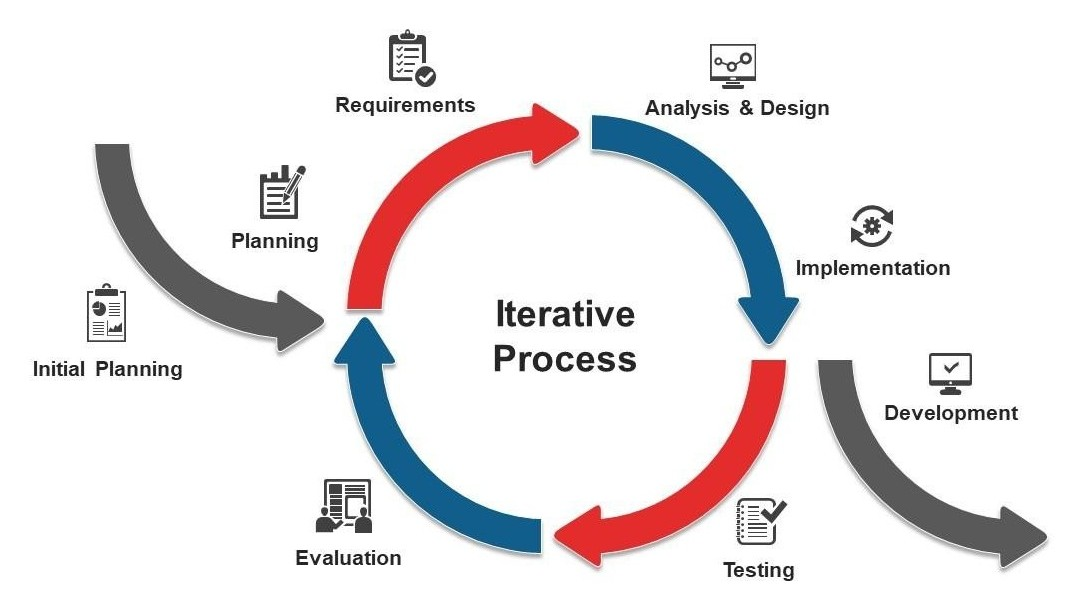
\includegraphics[width=15cm]{iterative_process_model}
	\caption{Iterative Process Model}
\end{figure}

\subsection{Initial Planning}

In this initial planning stage, the project goals and initial requirements are outlined. Key activities include:

\textbf{Defining Project Goals}: Setting the overall goals and vision for the "Track My Shop" application.

\textbf{Preliminary Requirement Analysis}:
Performing an initial analysis of high-level requirements and constraints.

\subsection{Planning}

The planning stage involves planning the upcoming iteration and setting specific goals for it. Key activities include:

\textbf{Setting Iteration Goals}:
Defining the objectives and outcomes for the current iteration.

\textbf{Identifying Resources}:
Allocating the necessary resources, including manpower, technology, and tools, for the iteration.

\subsection{Requirements Analysis and Design}

In this stage, detailed requirements are gathered and analyzed, and the system's design is conceptualized. Key activities include:

\textbf{Requirements Refinement}:
Analyzing and refining requirements based on feedback from previous iterations and stakeholders.

\textbf{System Design}:
Conceptualizing the system's design and architecture based on the refined requirements.

\subsection{Implementation and Development}

The implementation stage involves writing code and developing the iteration. Key activities include:

\textbf{Coding and Development}:
Writing the code based on the design and architecture defined in the previous stage.

\textbf{Integration}:
Integrating the developed components and modules into a cohesive iteration.

\subsection{Testing}

The testing stage involves validating the functionality and performance of the developed iteration. Key activities include:

\textbf{Functional Testing}:
Ensuring that the iteration meets the specified functional requirements.

\textbf{User Acceptance Testing (UAT)}:
Engaging users to validate the iteration against their expectations and requirements.

\subsection{Evaluation}

The evaluation stage involves assessing the outcomes of the iteration. Key activities include:

\textbf{Evaluation of Goals}:
Evaluating whether the iteration goals were achieved and identifying areas for improvement.

\subsection{Summary}

The iterative process model is adopted in the development of the "Track My Shop" application, allowing for incremental development, feedback incorporation, and continuous improvement. Each iteration adds new features, refines existing functionalities, and incorporates feedback for an improved and user-centric product.






\section{Architecture Overview}


\begin{figure}[h]
	\subsection{Entity Relationship Diagram (ERD) }
	\centering
	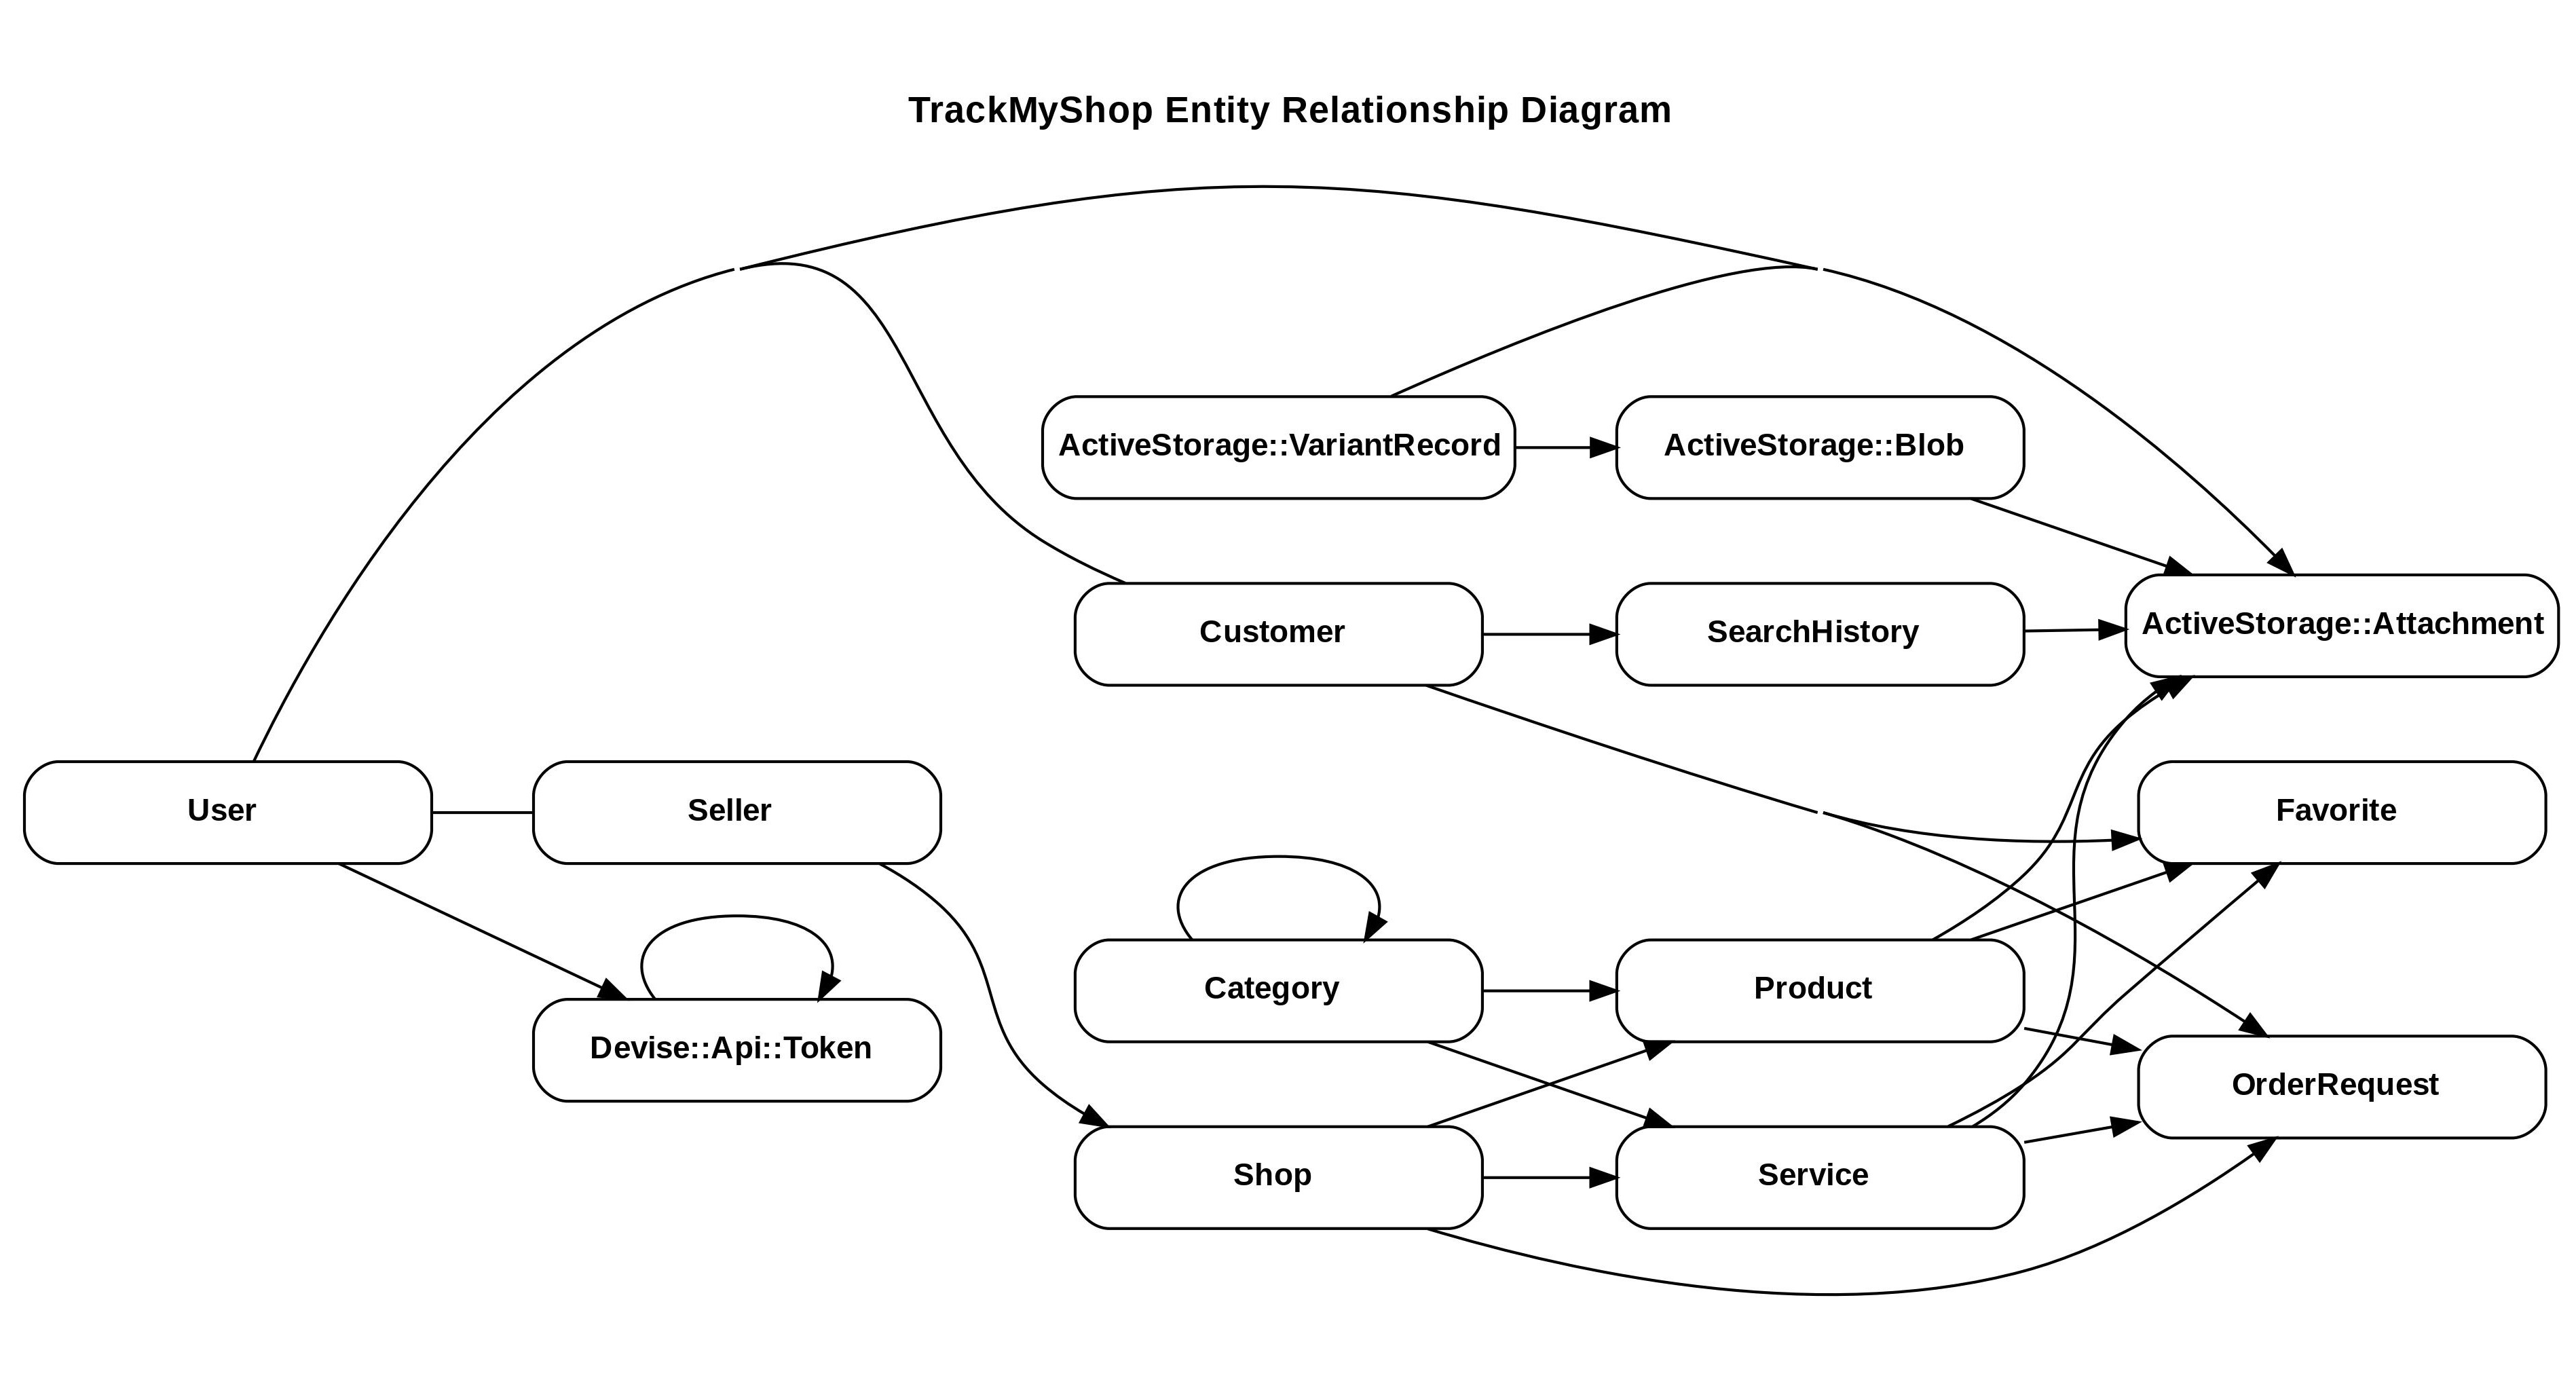
\includegraphics[width=17cm]{Entity-Relationship_Diagram}
	\caption{Track My Shop - Entity Relationship Diagram}
\end{figure}


\begin{figure}[h]
	\subsection{Class Diagram (UML) }
	\centering
	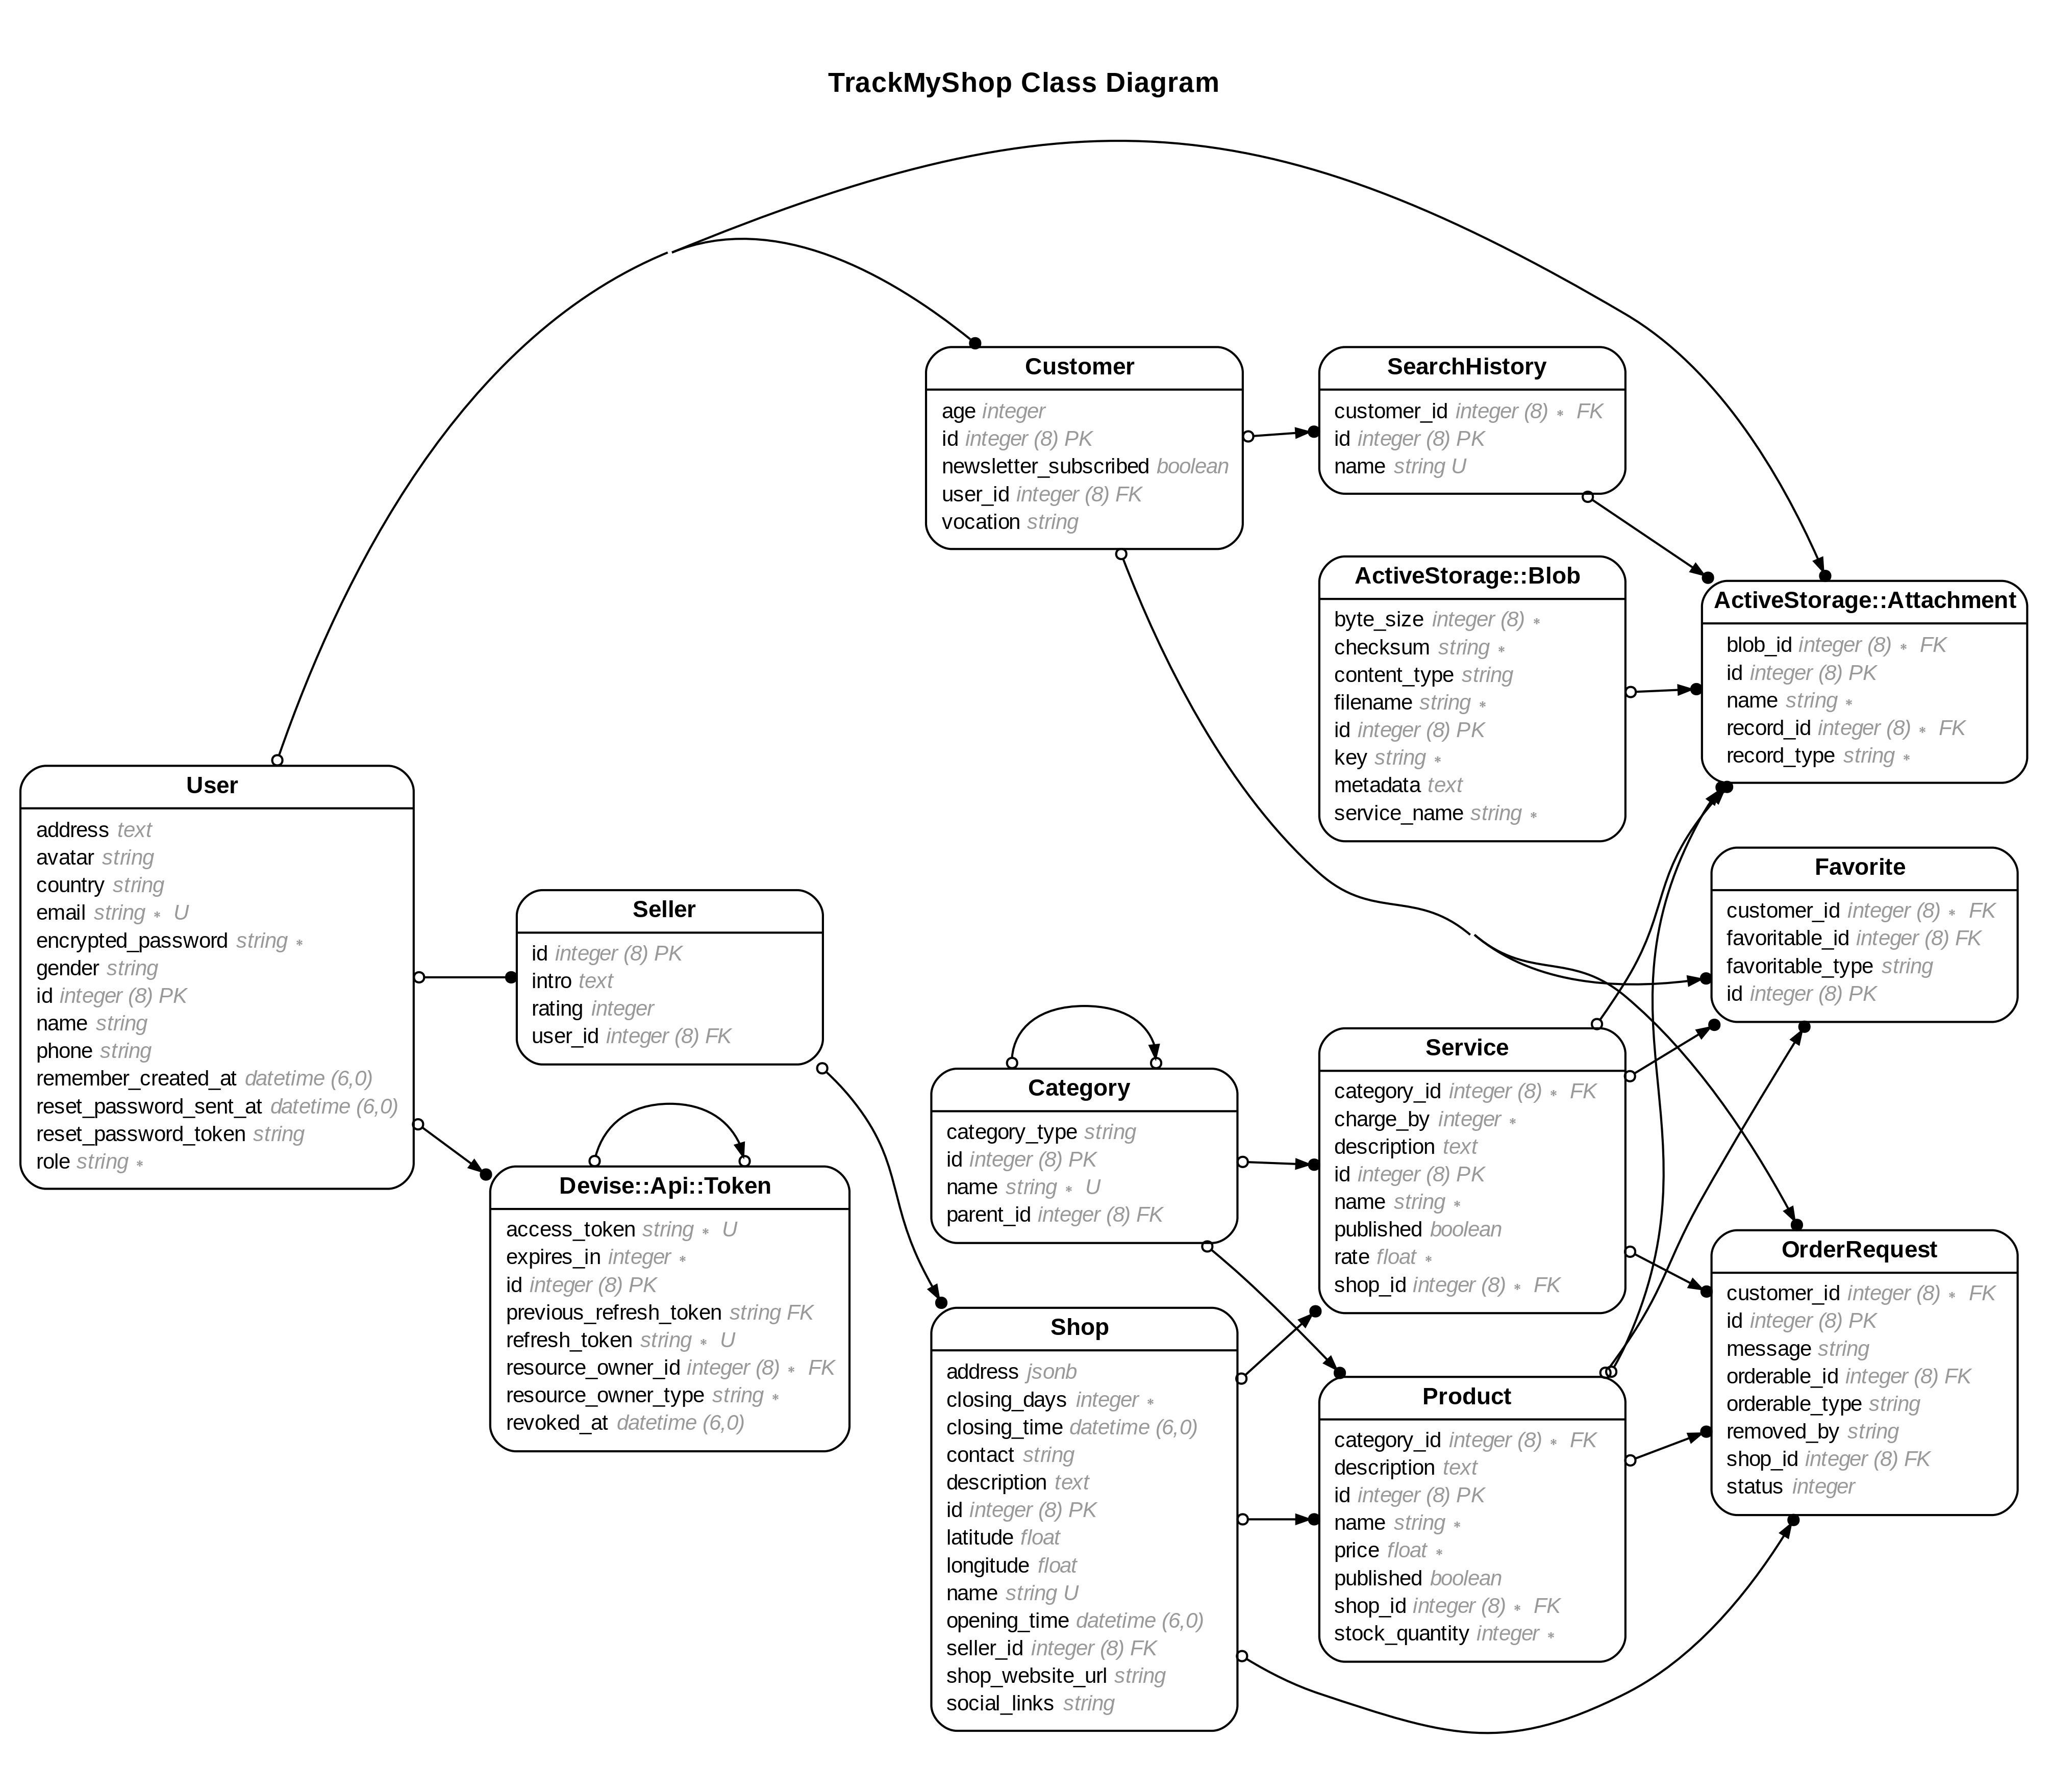
\includegraphics[width=17cm]{TrackMyShop_CD}
	\caption{Track My Shop - Class Diagram}
\end{figure}



\begin{figure}[h]
	\section{Design Description}
	Here is the basic architectural design of the Web Application:\\
	\centering
	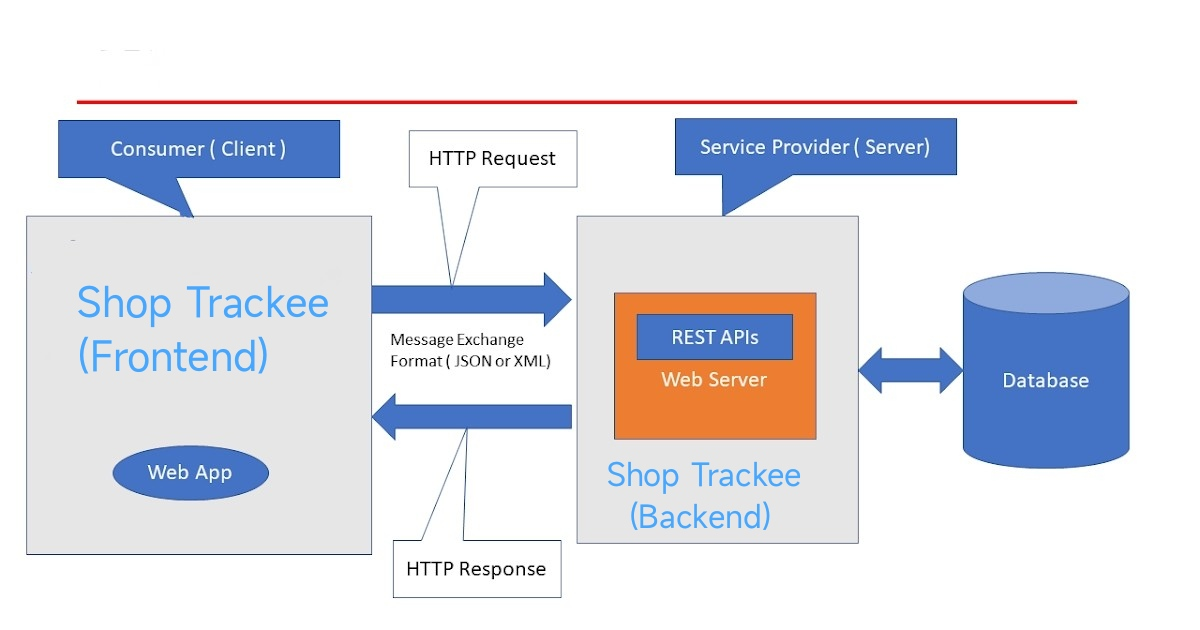
\includegraphics[width=1\linewidth]{design-description}
	\caption{Track My Shop - Design Description}
\end{figure}




% Chapter 4

\chapter{Implementation and Evaluation} % Main chapter title

\label{Chapter4} % For referencing the chapter elsewhere, use \ref{Chapter1}

\lhead{Chapter 4. \emph{Implementation and Evaluation}} % This is for the header on each page - perhaps a shortened title

%----------------------------------------------------------------------------------------
\section{Development Stages }
Following are the stages of development:
\subsection{Strategy Stage}
We designed our web application while keeping in mind the requirements of our end sellers and customers. In order to make it a success we planned each and everything beforehand. We have learned our users demand and then planned our project on it. We have designed it in such a way that it can be easy to use and handle. After jotting down our requirements we made diagrams so that it can give an outlook of our system. After this we worked on our database and later on its implementation. We also wrote the project code, then we integrated and tested our it to verify if its working.

\section{Implementation}
Following is described about the implementation level things:

\subsection{Tools and Technologies}
\begin{enumerate}
	\item Server-Side API Framework \textbf{Ruby on Rails}
	\item Front-End Frameworks:
	\begin{itemize}
		\item \textbf{Next.js} (framework built on REACT Js library)
		\item \textbf{Bootstrap5} (CSS framework)
		\item \textbf{Google Material UI} (for interactive components)
		\item \textbf{Google Maps API}
	\end{itemize}
	\item DBMS \textbf{PostgreSQL}
	\item Version Control System (VCS): \textbf{Git, Github}
	\item Integrated Development Environment (IDE): \textbf{RubyMine, VS Code}
	\item API and Web testing tool: \textbf{Postman}
	\item Data Caching server: \textbf{Redis}
	\item Hosting Service for API: \textbf{Heroku}
	\item Hosting Service for Front-End App: \textbf{Amazon Static Hosting S3}
	\item CI | CD tool: \textbf{Github Actions}
	\item Media Storage Service: \textbf{AWS S3}
	\item Image Recognition Service: \textbf{AWS Rekognition}
	\item Domain Name Service: \textbf{AWS Route53}
	\item Domain Platform: \textbf{Namecheap.me}
	\item Bug Report Service: \textbf{Sentry}
	\item Mailer Service: \textbf{Mailjet}
	
\end{enumerate}

\section{System Integration}
System integration in the "Track My Shop" project is a critical process where all the individual components and modules of the system are combined and tested to ensure they function as a unified, cohesive unit. This integration involves merging the backend functionalities, including database management and server operations, with the frontend user interface to create a seamless and functional application. The integration process also incorporates third-party services, such as image recognition, mapping APIs and Deployment on AWS/Heroku, ensuring their proper interaction within the application. Rigorous testing and validation are conducted to confirm that the integrated system operates smoothly, with data flowing seamlessly between various components.\\
Achieving a successful integration is vital for delivering a reliable, efficient, and feature-rich web application that can be run on any environment and on any web browser, meets the needs and expectations of both sellers and customers. 

\section{User Interface}
The user interface (UI) of the "Track My Shop" project is crafted to deliver a seamless and engaging experience for both sellers and customers. Sellers are provided with a comprehensive dashboard offering insights into their shops, order requests, and sales statistics. They can efficiently manage their shop listings, adding new products/services and updating existing ones. On the other hand, customers are greeted with an intuitive interface that allows effortless browsing of nearby shops and their offerings, categorized for easy exploration. The search functionality is versatile, enabling customers to search by text, images, or based on their preferences. Clear product/service details, interactive maps for shop locations, easy order request processes, and a user-friendly profile management system further enhance the overall usability. The UI is designed to be accessible and responsive to various type of devices and user needs, ultimately fostering a positive and satisfying interaction for all users.
\newpage

\begin{figure}[h]
	\subsection{Login}
	\centering
	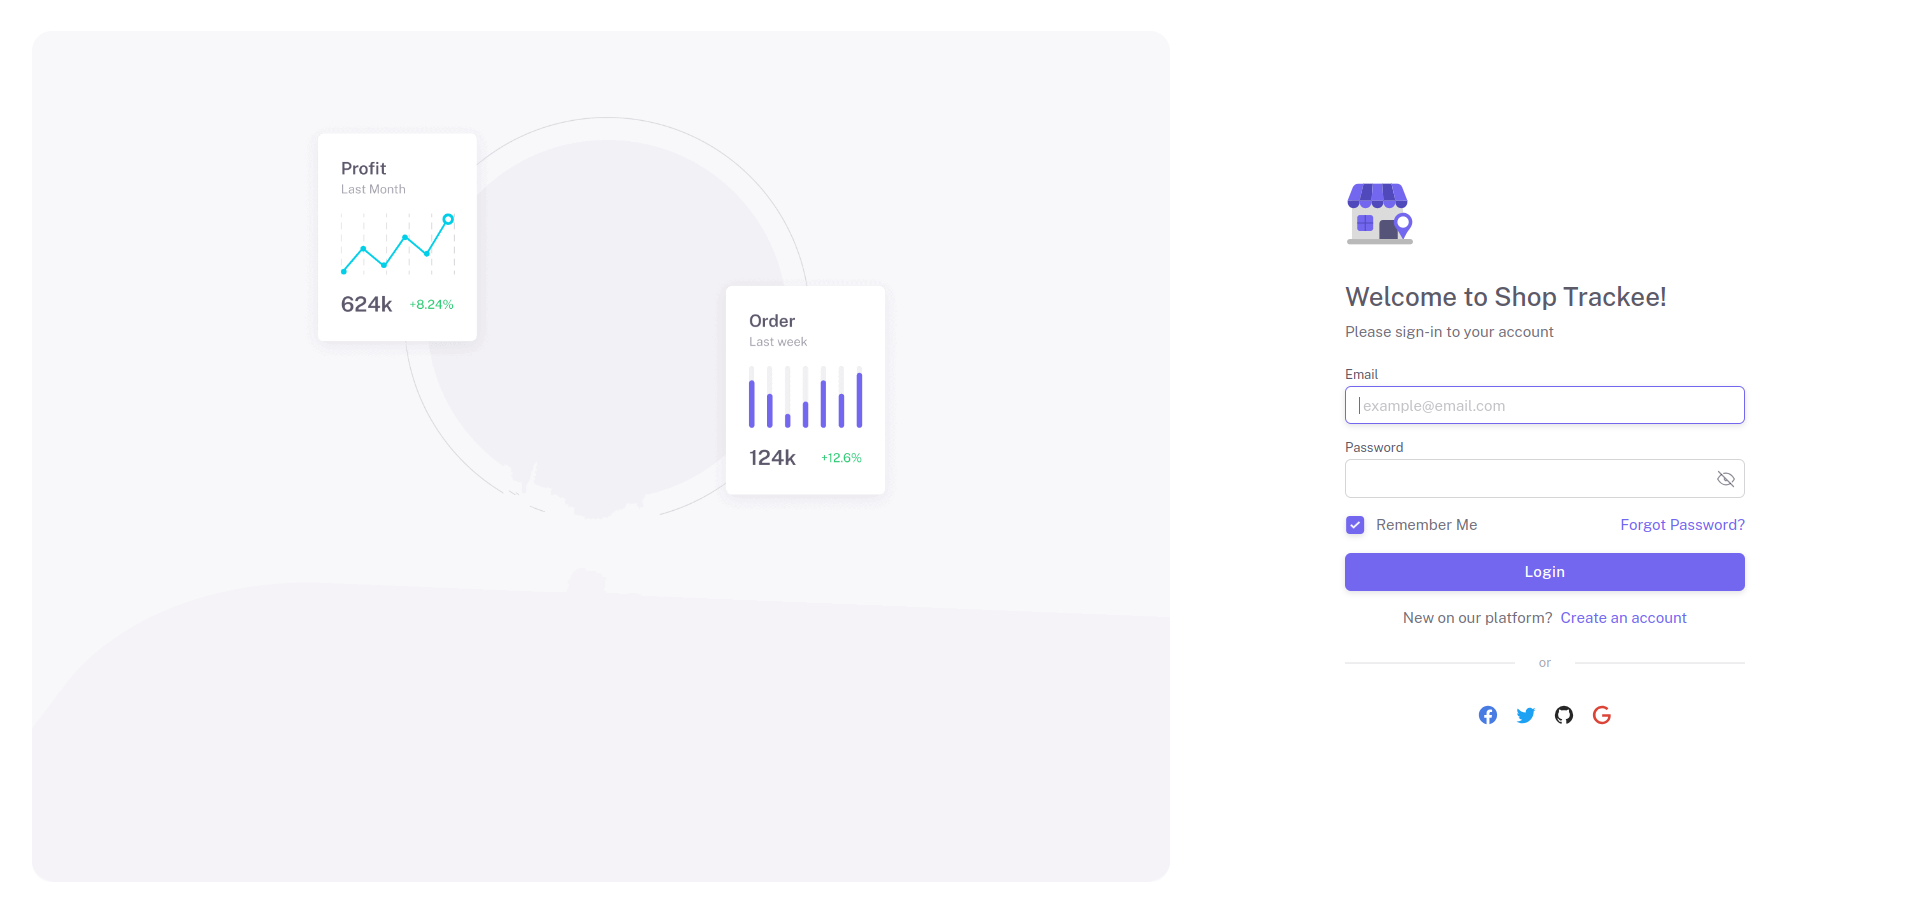
\includegraphics[width=1\textwidth]{login-page}
	\caption{Shop Trackee - Login}
\end{figure}

\begin{figure}[h]
	\subsection{Register}
	\centering
	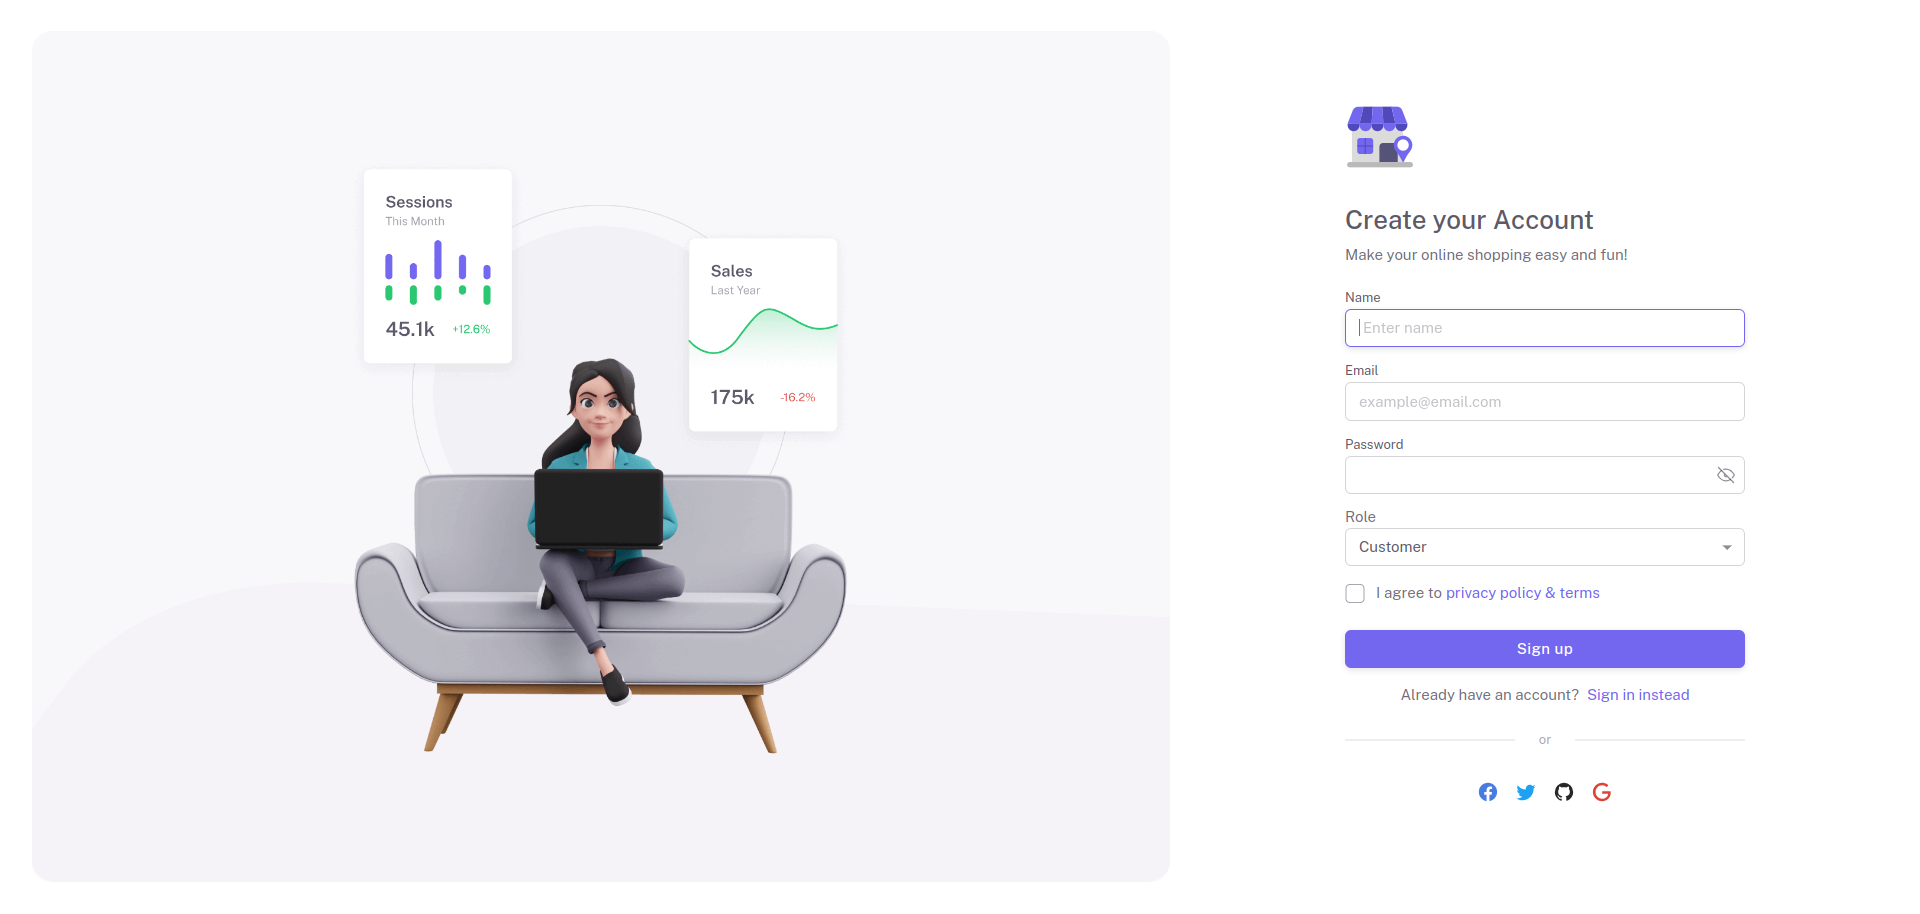
\includegraphics[width=1\textwidth]{signup-page}
	\caption{Shop Trackee - Register}
\end{figure}
\newpage

\begin{figure}[h]
	\subsection{Forgot Password}
	\centering
	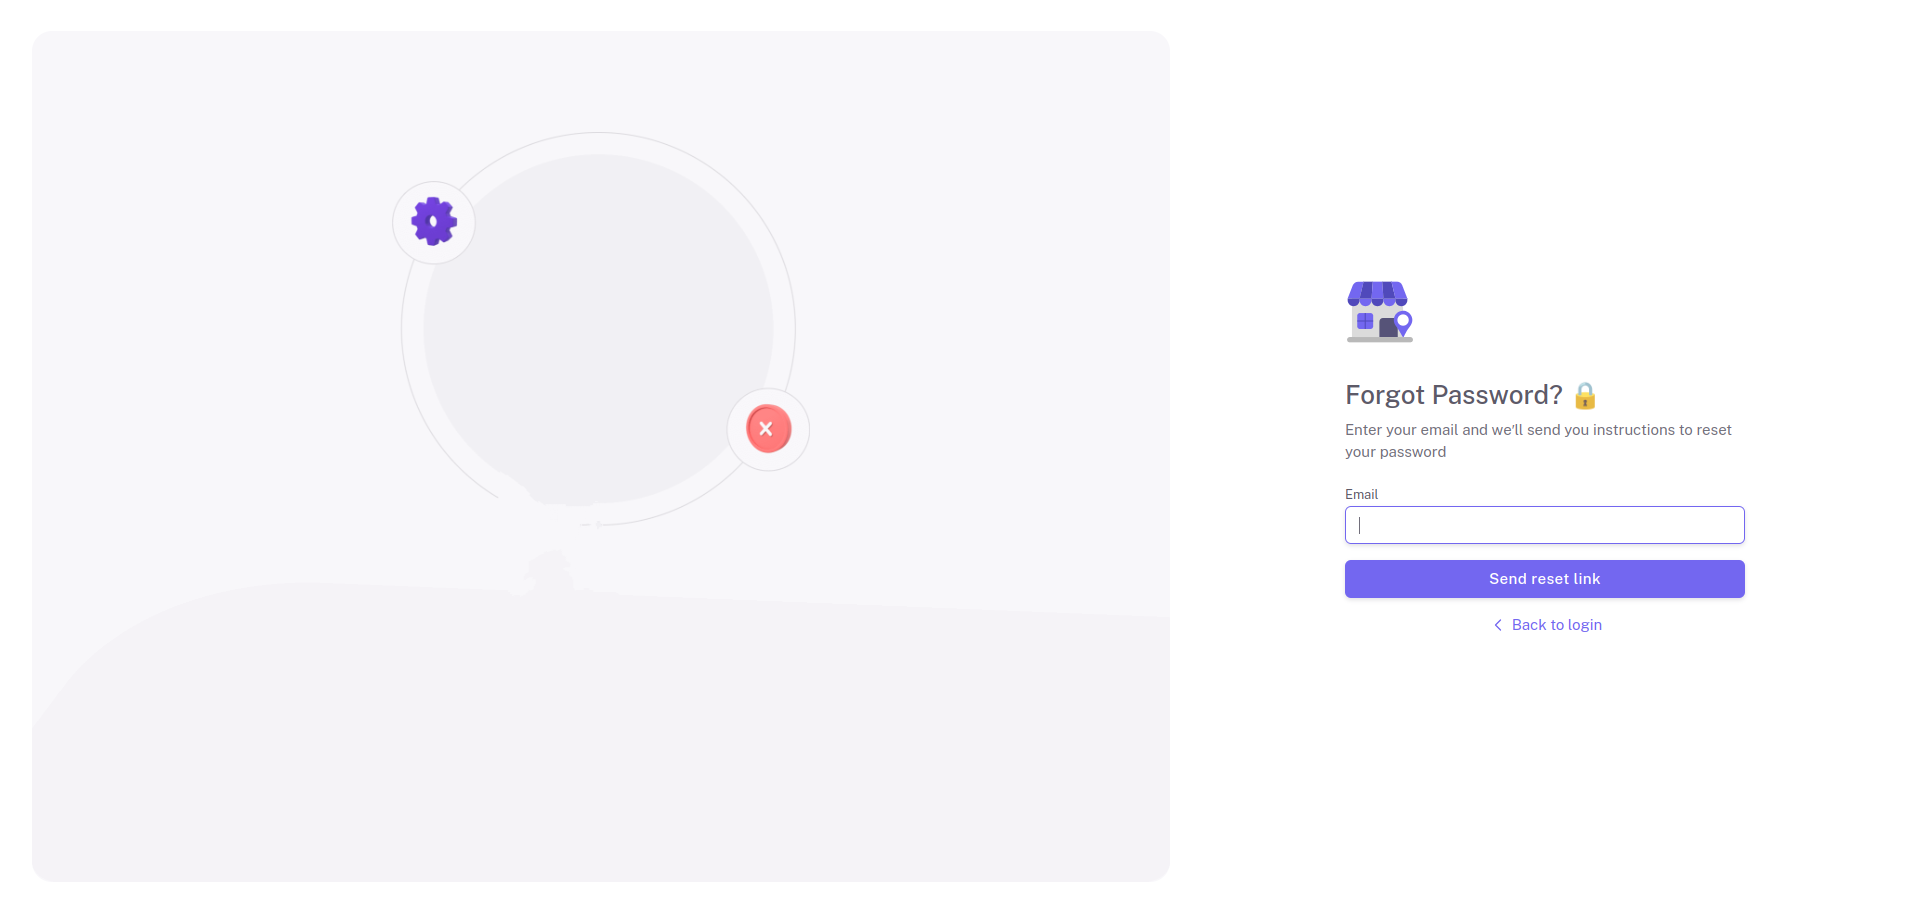
\includegraphics[width=1\textwidth]{forgot-password-page}
	\caption{Shop Trackee - Forgot Password}
\end{figure}

\begin{figure}[h]
	\subsection{Profile}
	\centering
	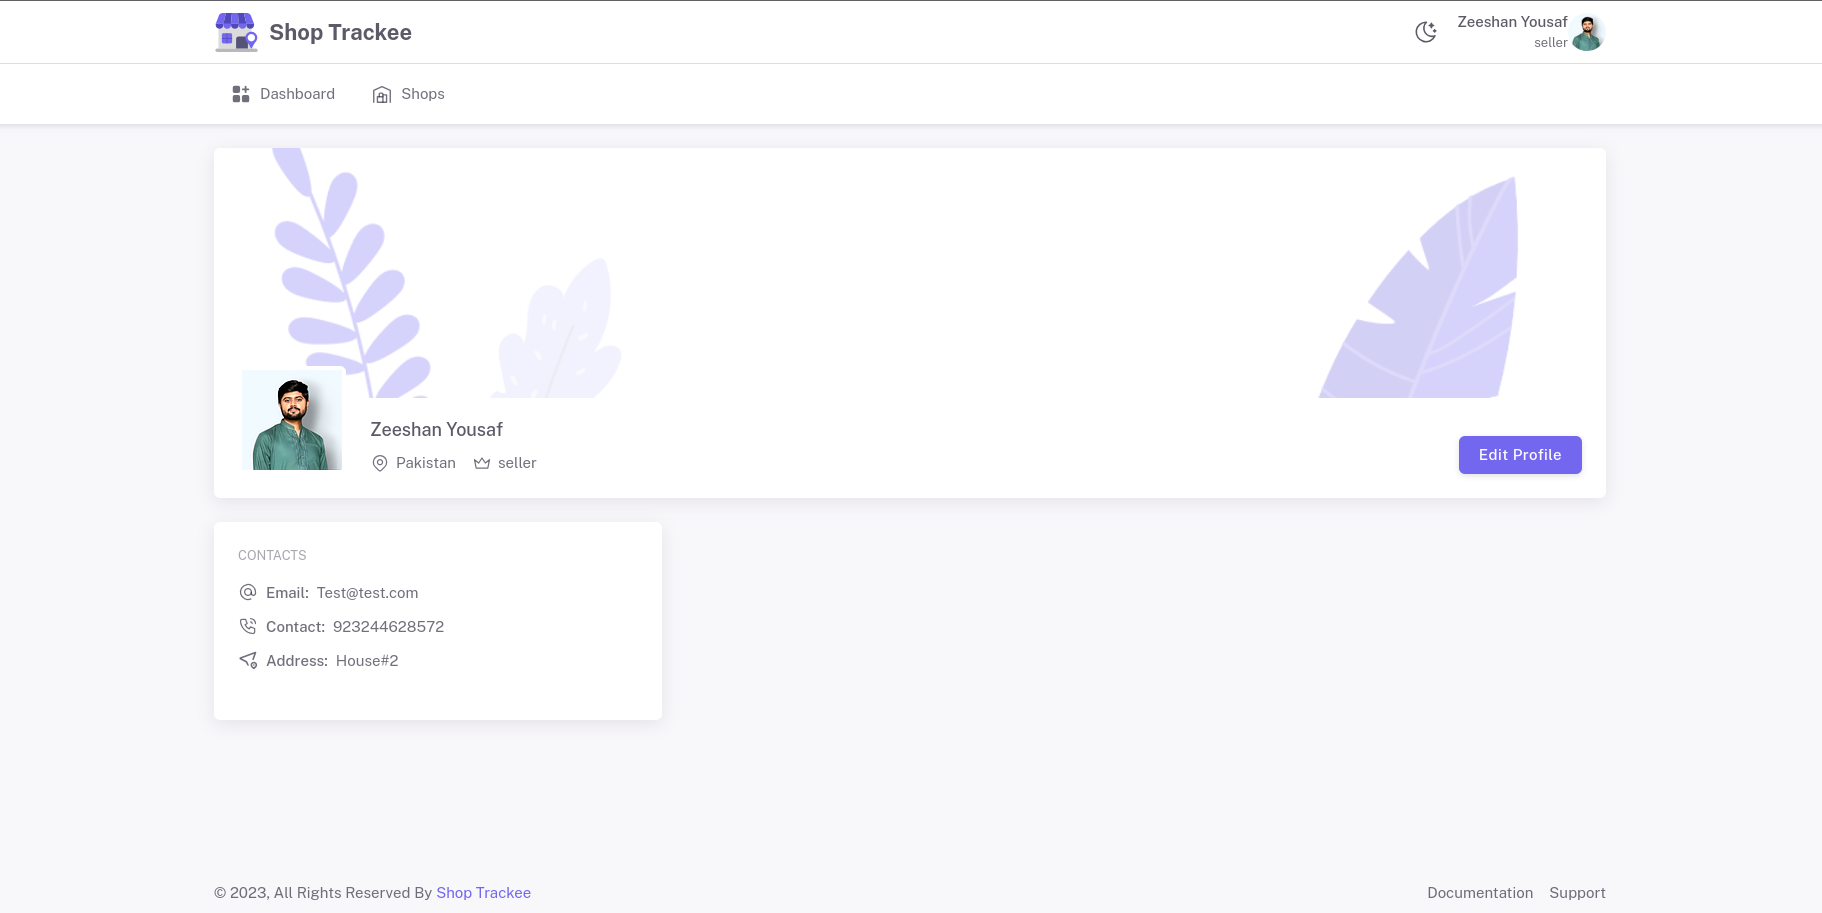
\includegraphics[width=1\textwidth]{seller-profile-page}
	\caption{Shop Trackee - Profile}
\end{figure}
\newpage

\begin{figure}[h]
	\subsection{Profile Edit}
	\centering
	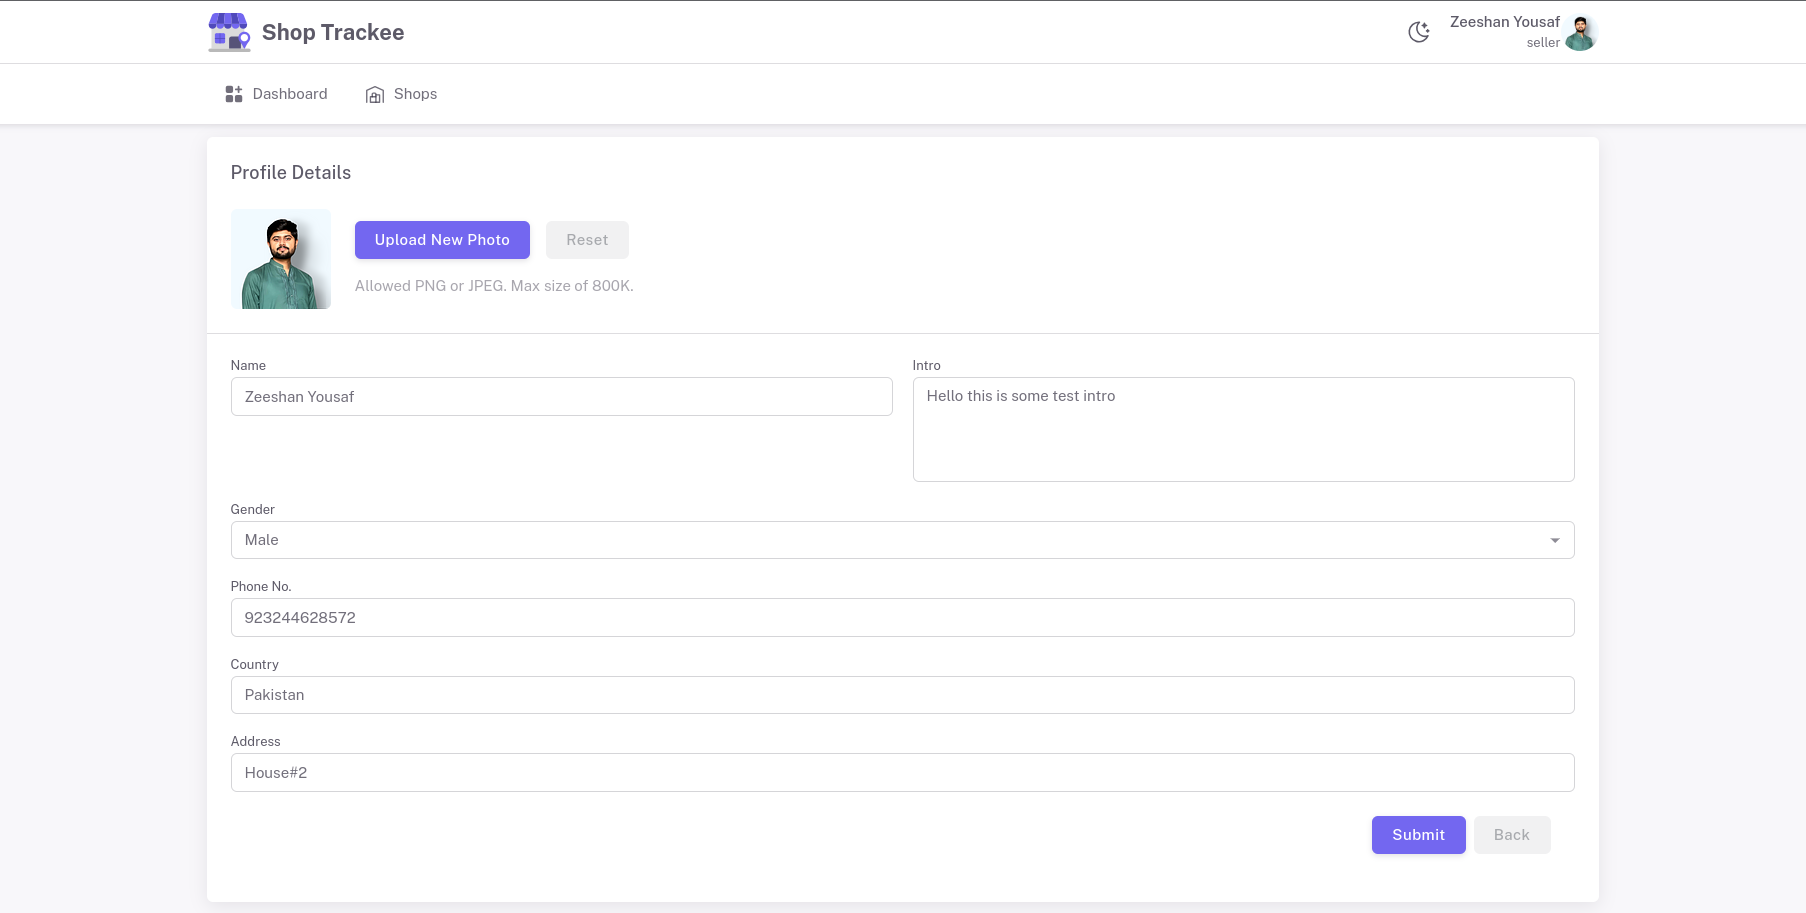
\includegraphics[width=1\textwidth]{profile-edit-page}
	\caption{Shop Trackee - Profile Edit}
\end{figure}


\begin{figure}[h]
	\subsection{Seller Dashboard}
	\centering
	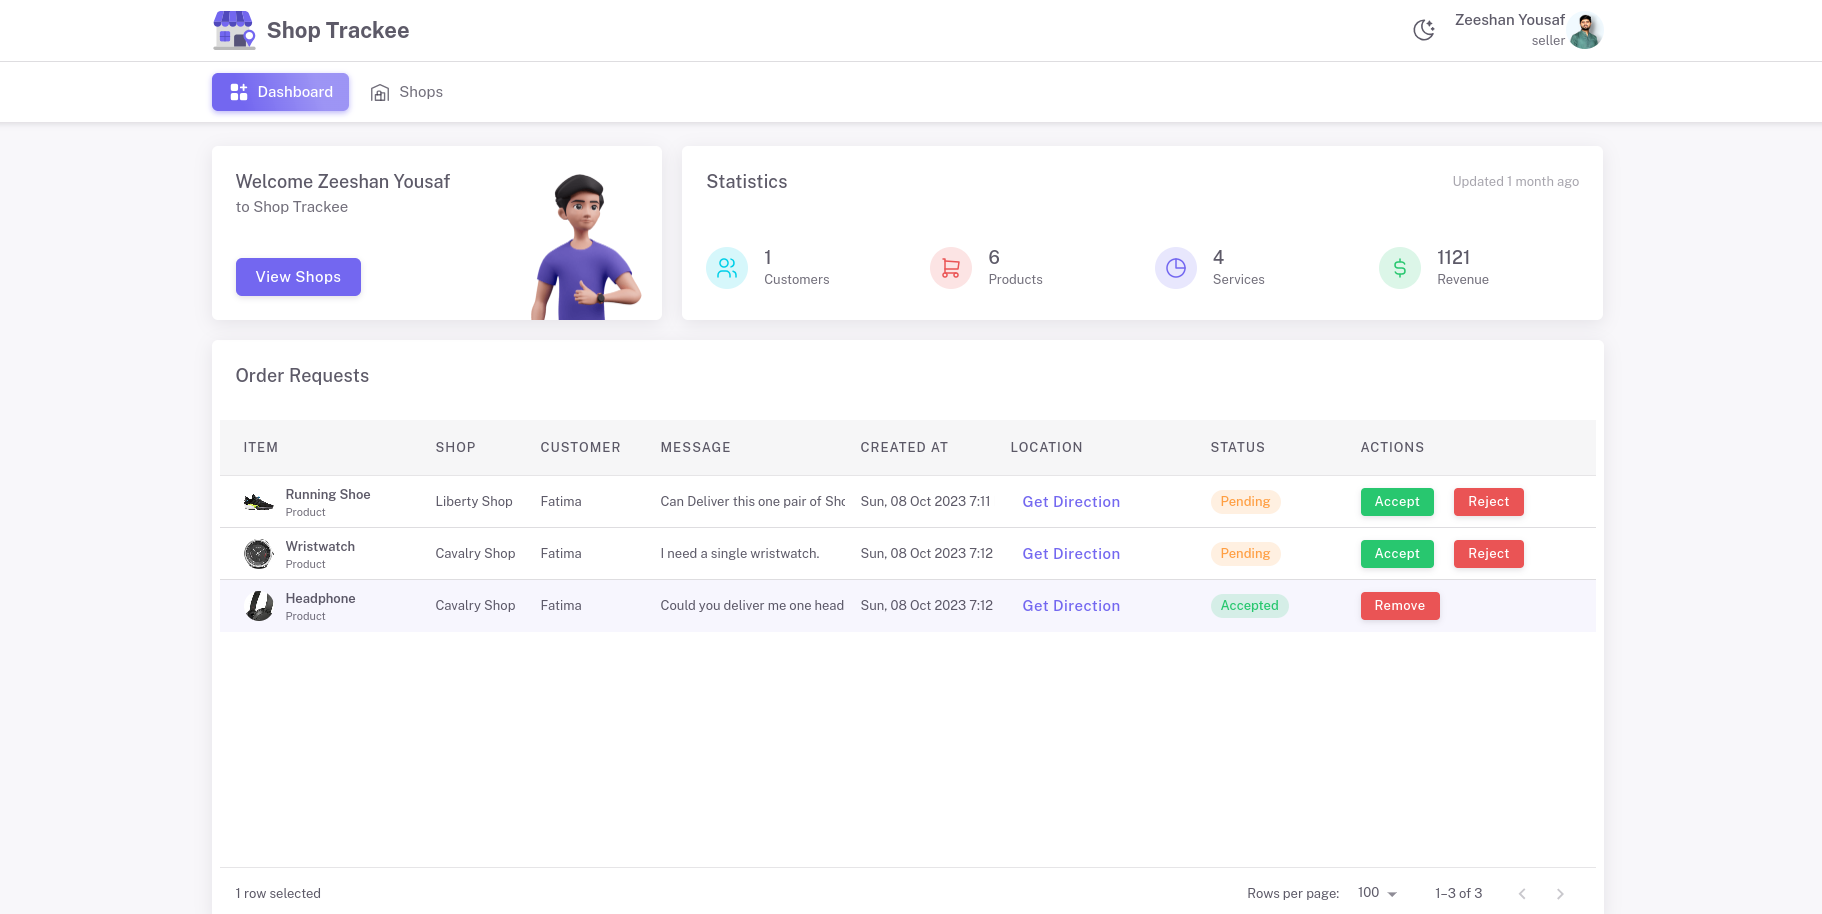
\includegraphics[width=1\textwidth]{seller-dashboard-page}
	\caption{Shop Trackee - Seller Dashboard}
\end{figure}
\newpage

\begin{figure}[h]
	\subsection{Seller Shops}
	\centering
	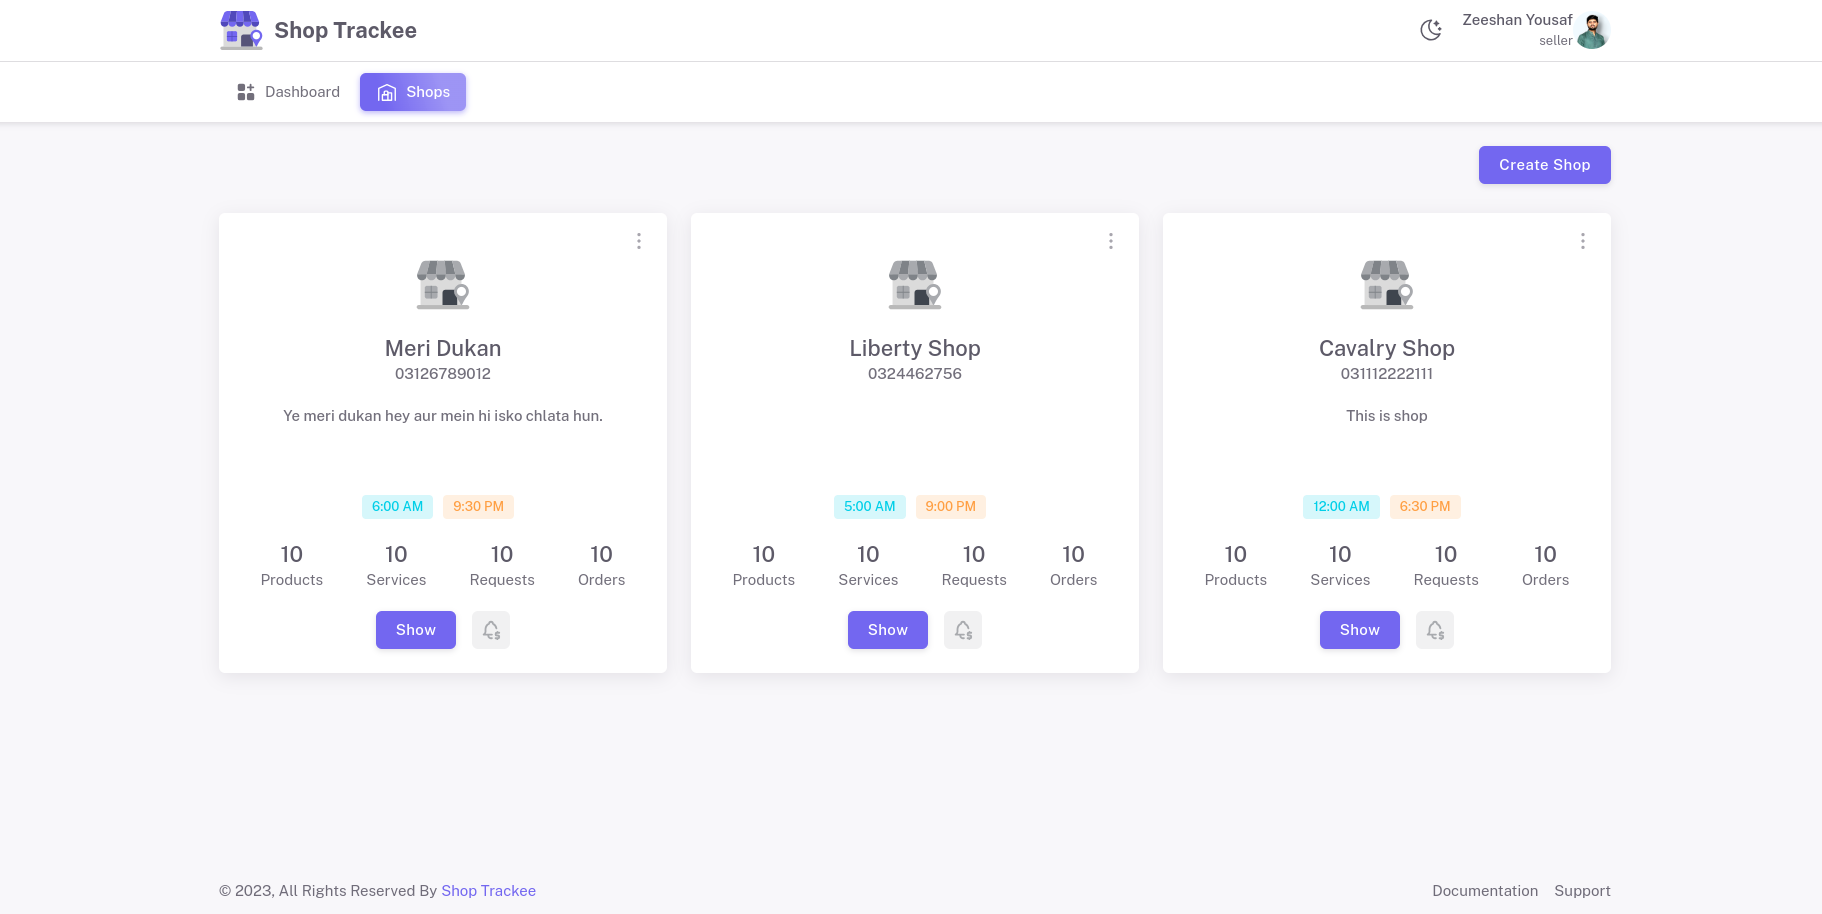
\includegraphics[width=1\textwidth]{seller-shops-page}
	\caption{Shop Trackee - Seller Shops}
\end{figure}

\begin{figure}[h]
	\subsection{Seller Shop Create}
	\centering
	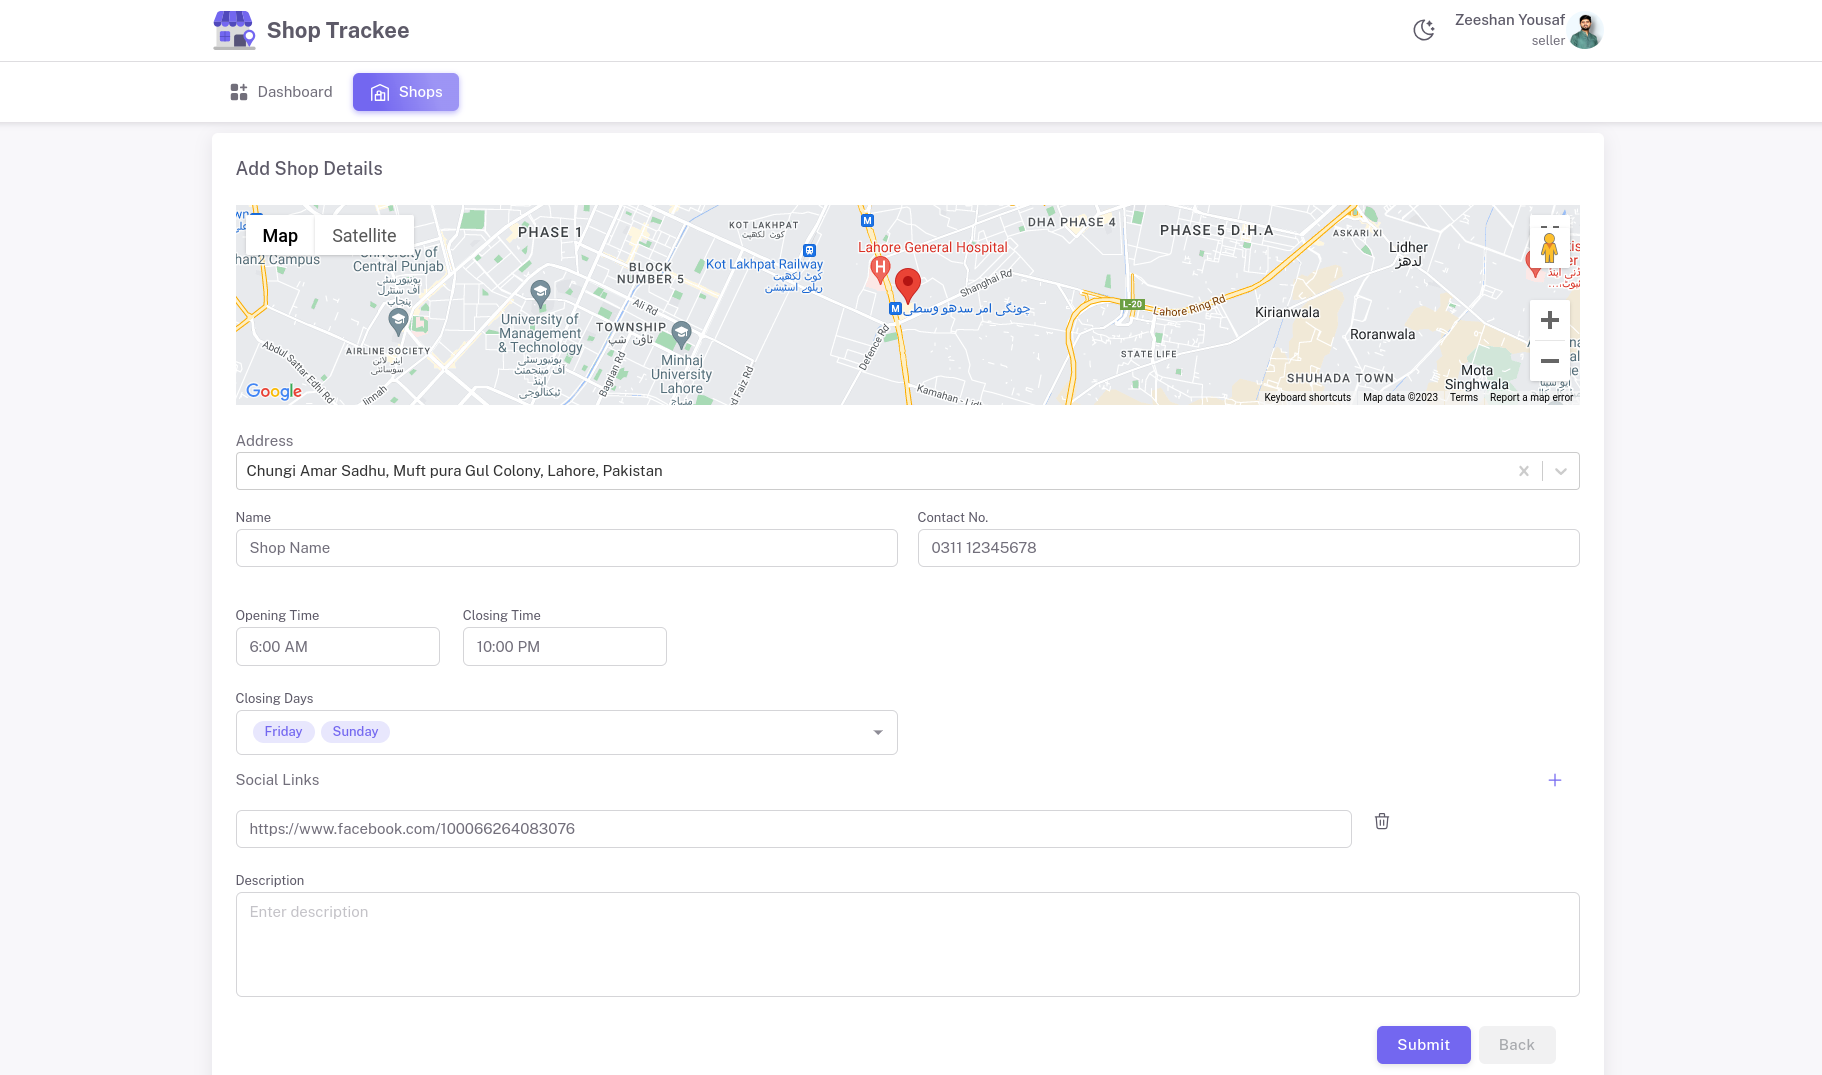
\includegraphics[width=0.9\textwidth]{seller-shop-create-page}
	\caption{Shop Trackee - Shop Create}
\end{figure}
\newpage

\begin{figure}[h]
	\subsection{Seller Add Product}
	\centering
	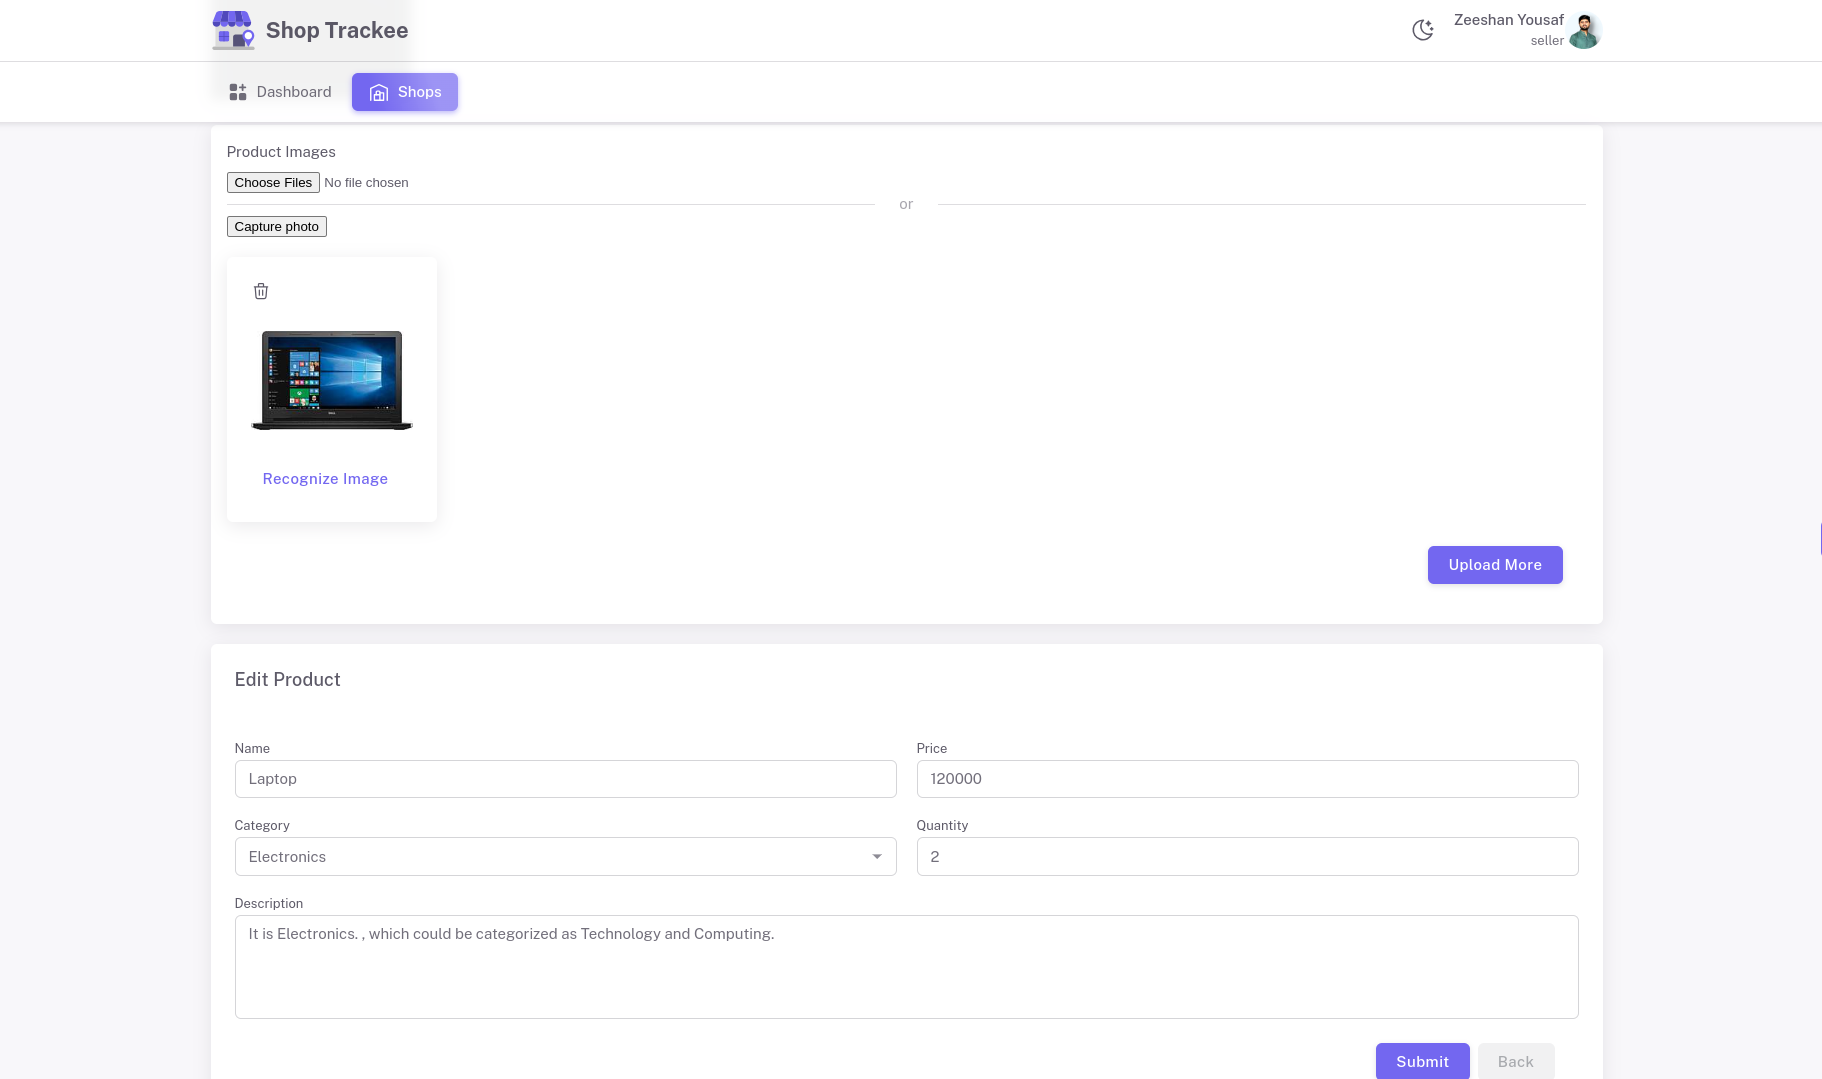
\includegraphics[width=1\textwidth]{product-form-page}
	\caption{Shop Trackee - Add Product}
\end{figure}

\begin{figure}[h]
	\subsection{Seller Add Service}
	\centering
	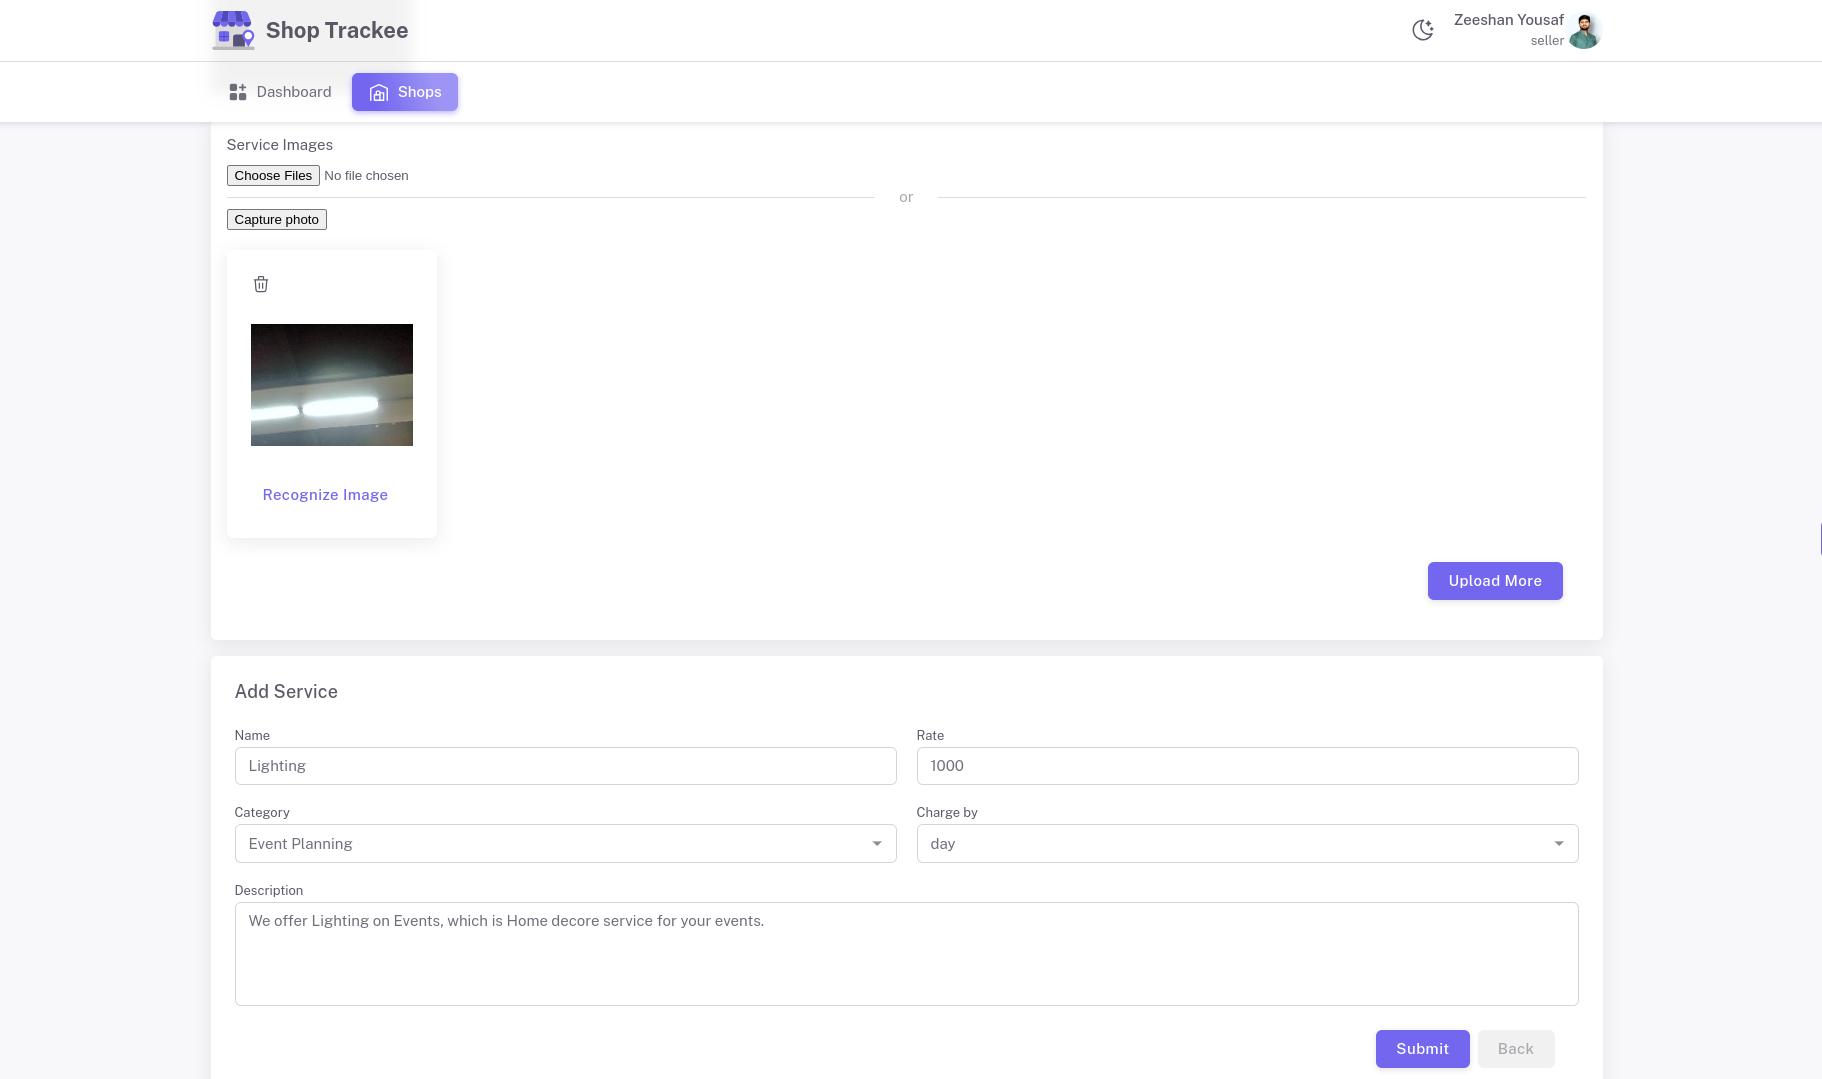
\includegraphics[width=0.9\textwidth]{service-form-page}
	\caption{Shop Trackee - Add Service}
\end{figure}
\newpage

\begin{figure}[h]
	\subsection{Seller Products and Services Listing}
	\centering
	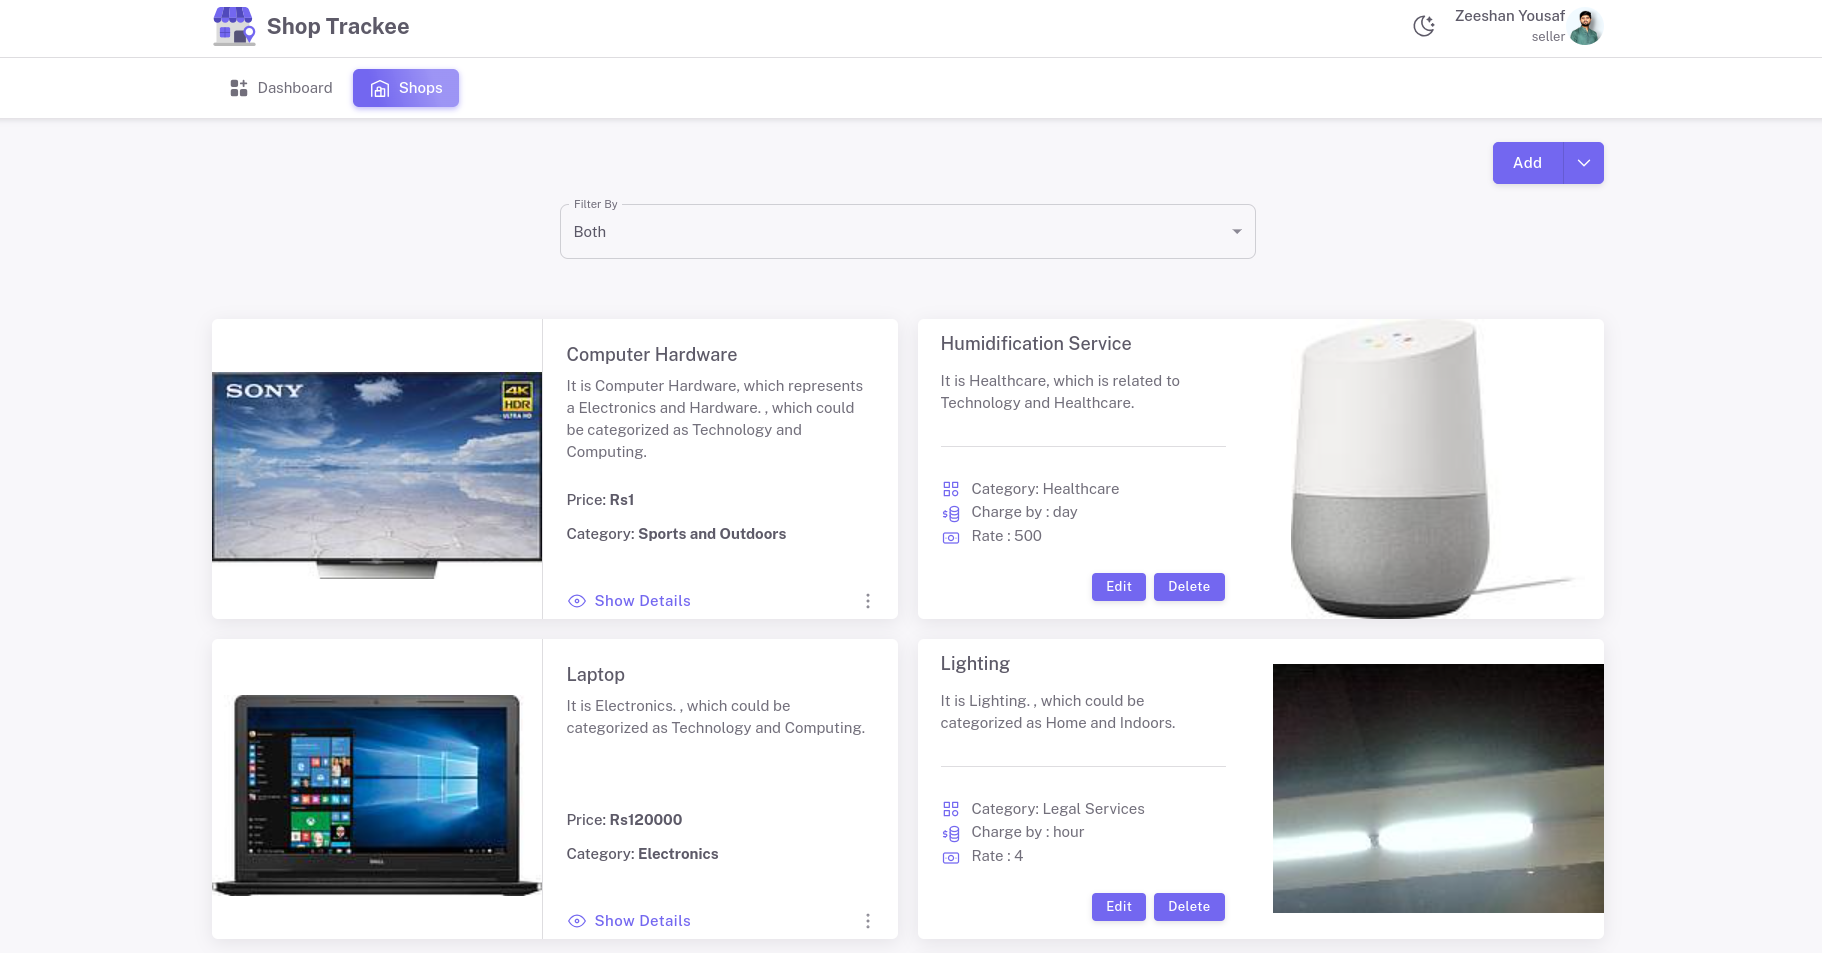
\includegraphics[width=1\textwidth]{products-services-page}
	\caption{Shop Trackee - Products and Services Listing}
\end{figure}


\begin{figure}[h]
	\subsection{Customer Home}
	\centering
	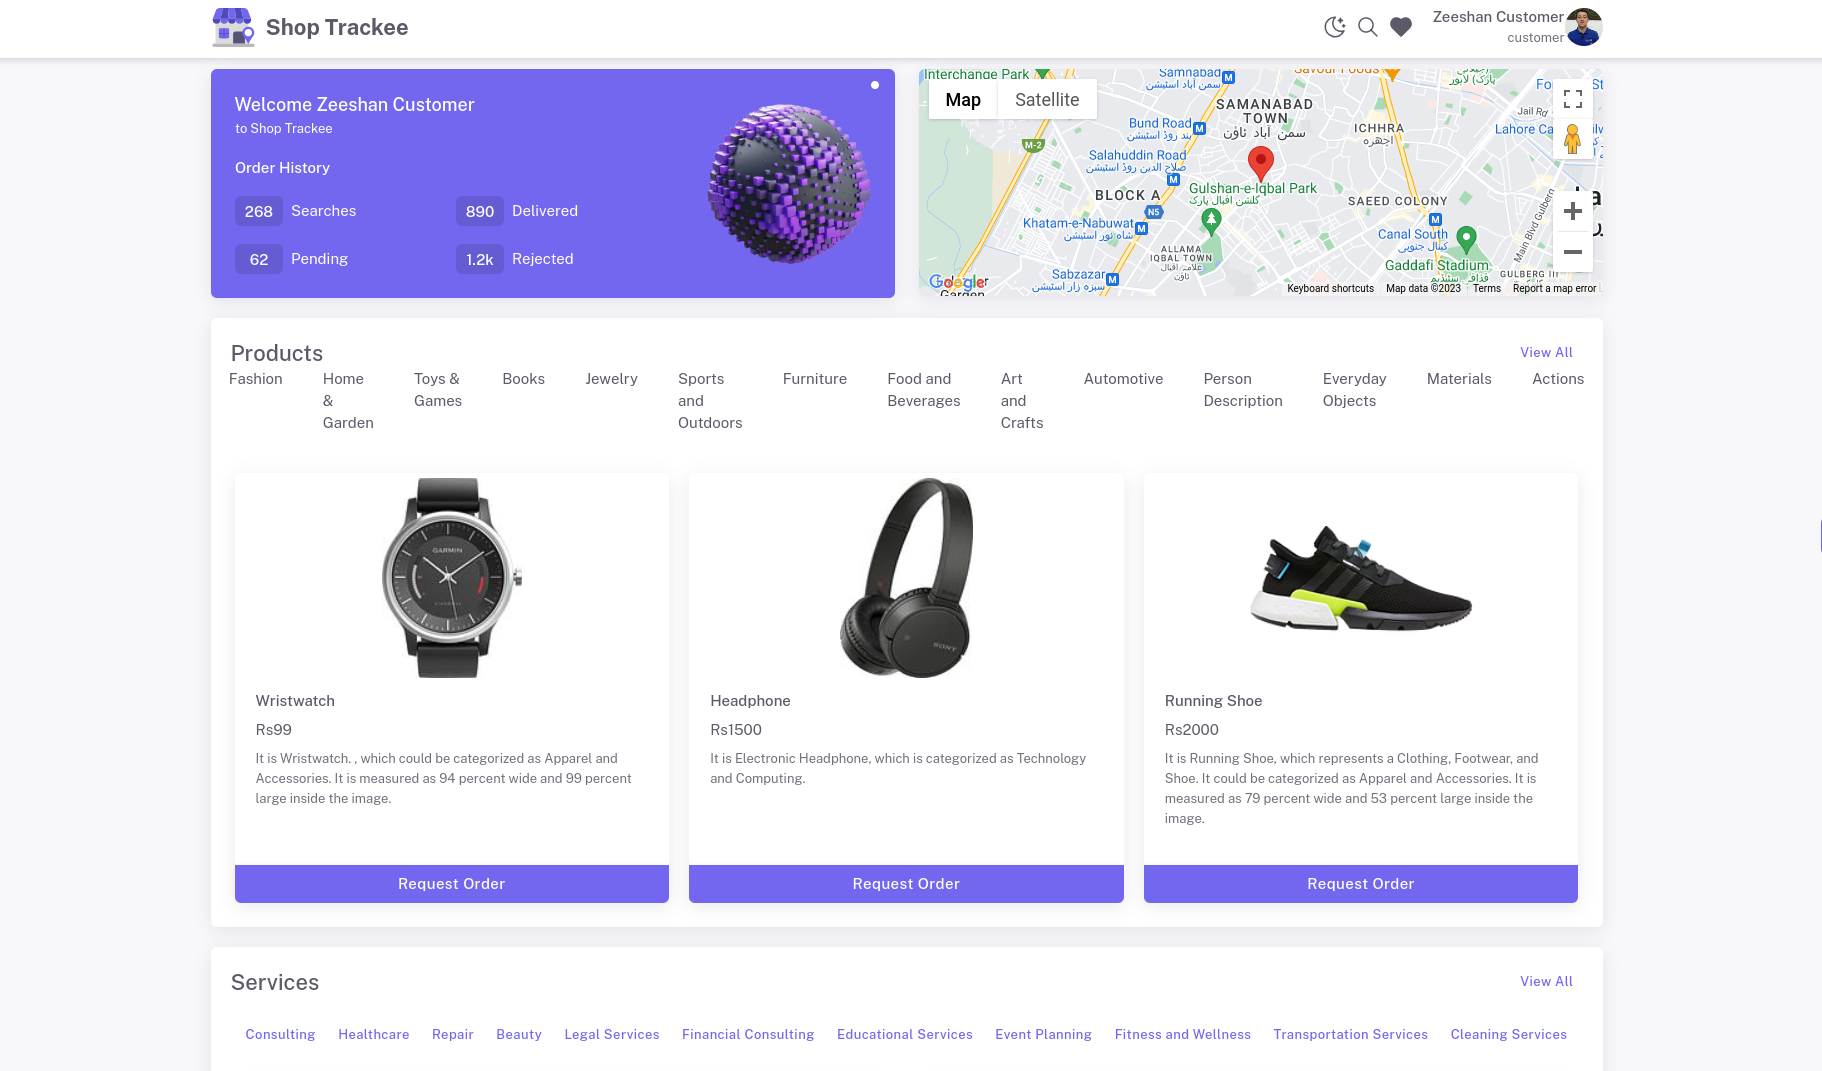
\includegraphics[width=1\textwidth]{customer-home-page}
	\caption{Shop Trackee - Customer Home}
\end{figure}
\newpage

\begin{figure}[h]
	\subsection{Customer Searching Around}
	\centering
	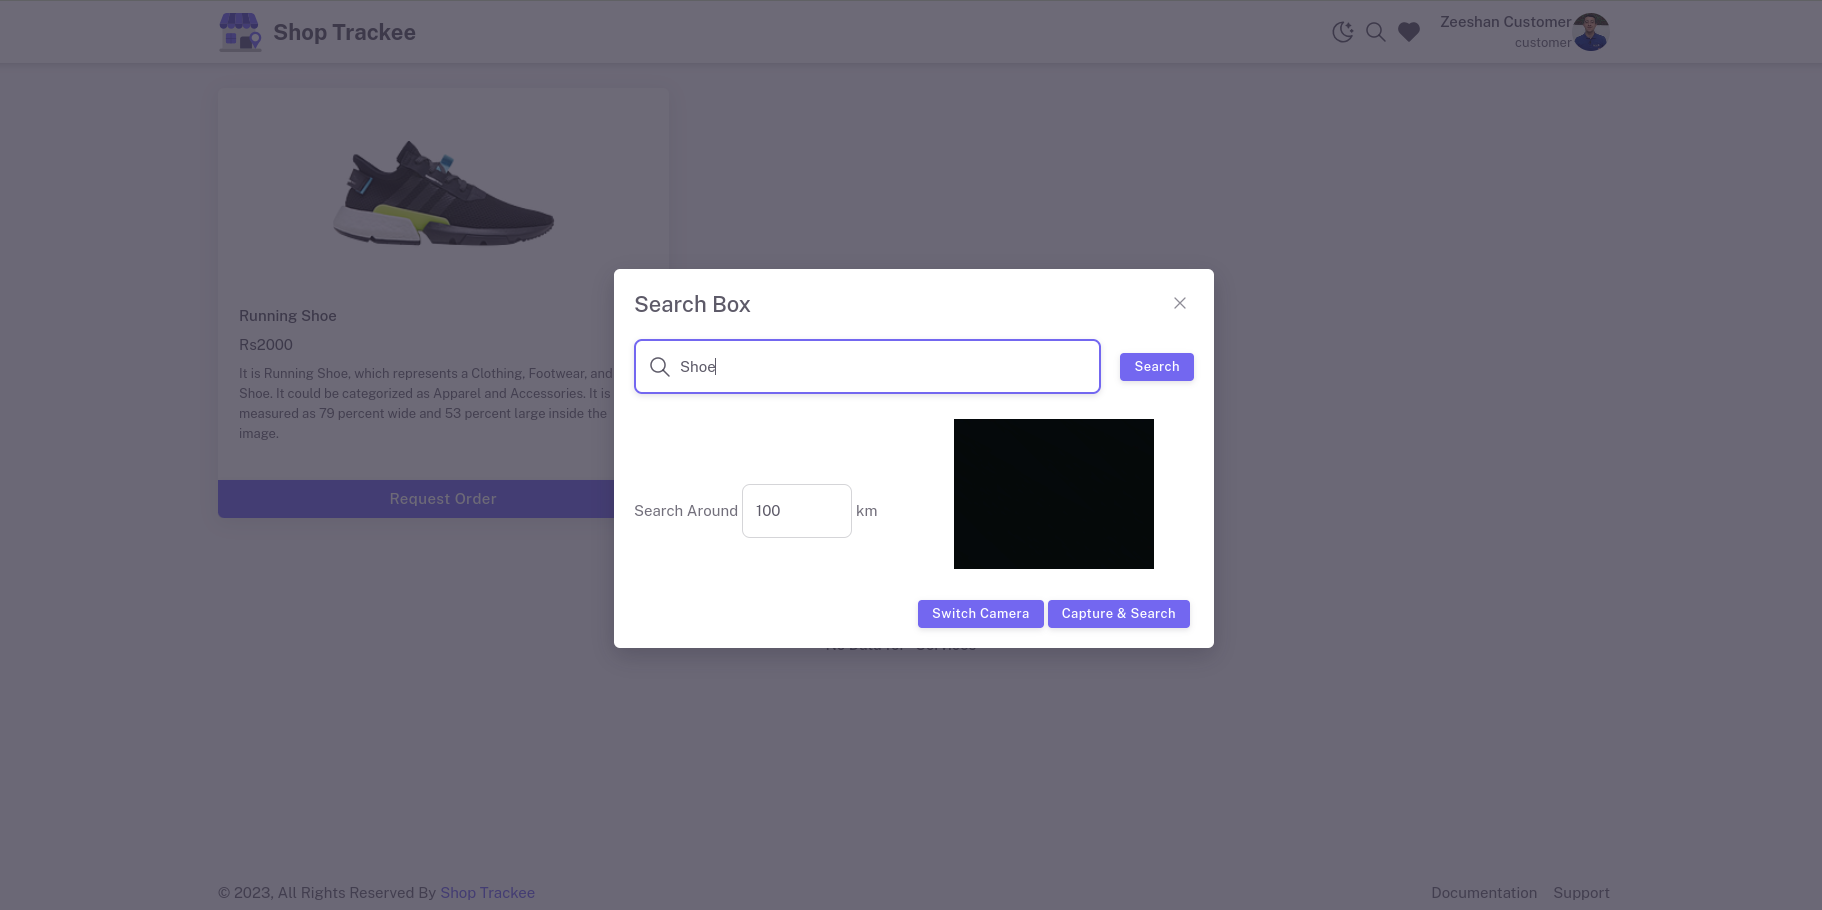
\includegraphics[width=1\textwidth]{searching-page}
	\caption{Shop Trackee - Customer Searching Around}
\end{figure}


\begin{figure}[h]
	\subsection{Customer Requesting Order}
	\centering
	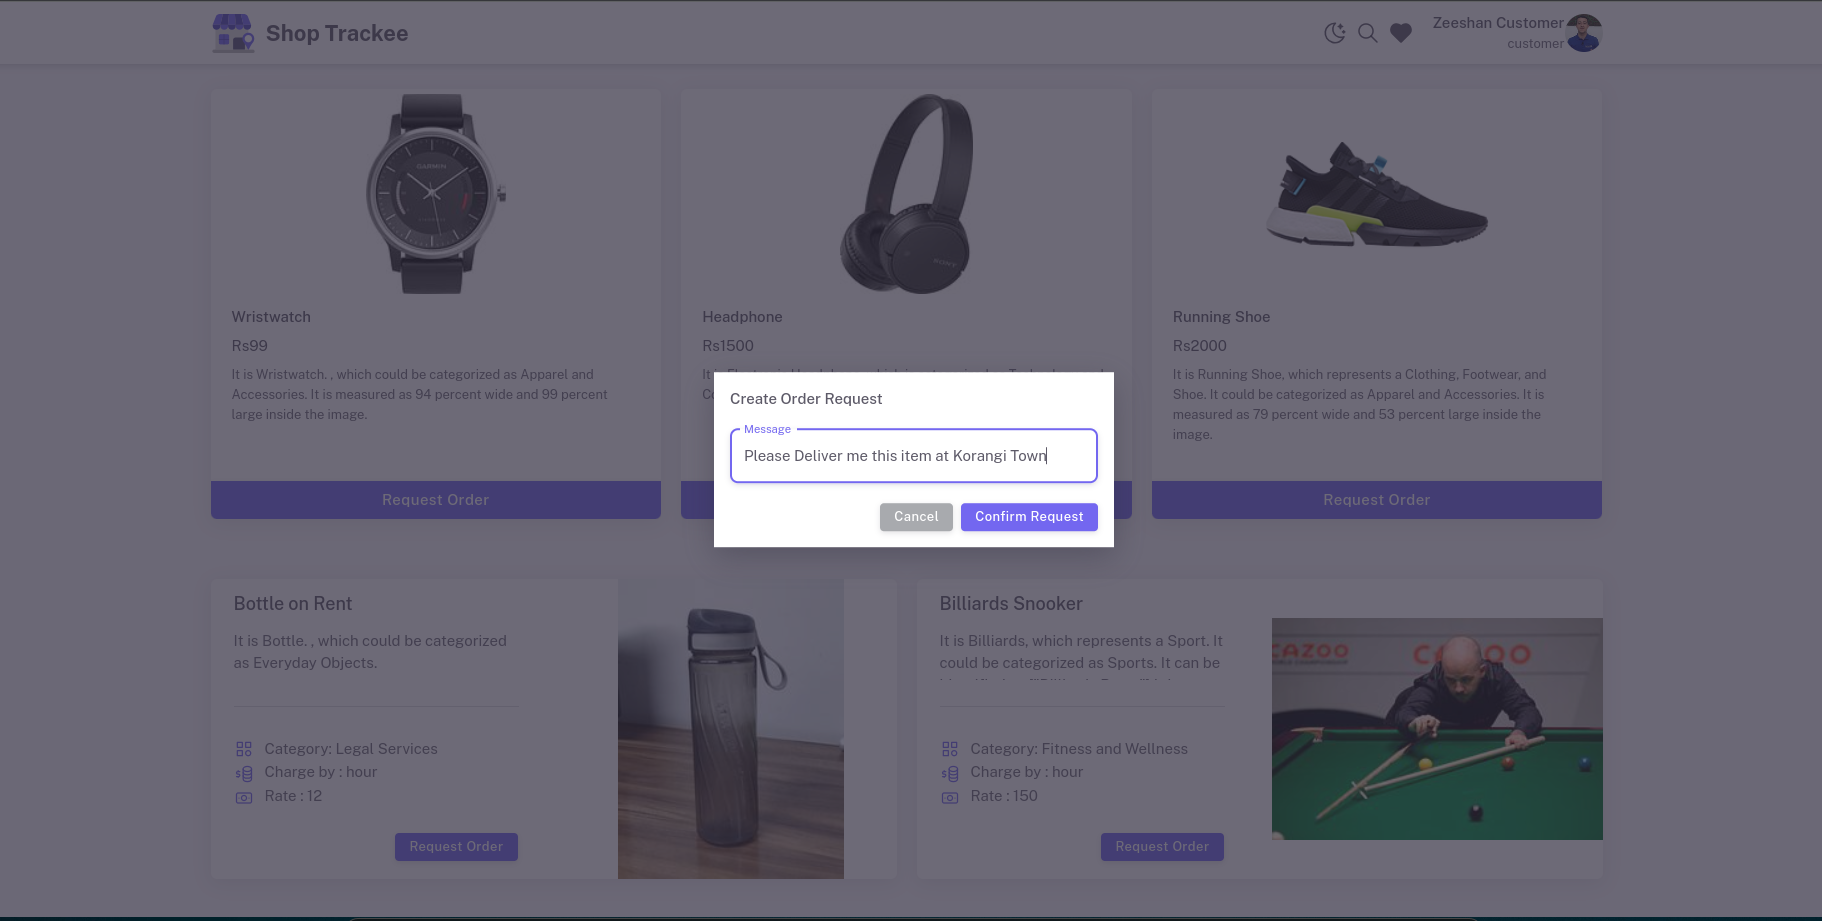
\includegraphics[width=1\textwidth]{requesting-order-page}
	\caption{Shop Trackee - Customer Requesting Order}
\end{figure}
\newpage

\begin{figure}[h]
	\subsection{Customer Order Requests History}
	\centering
	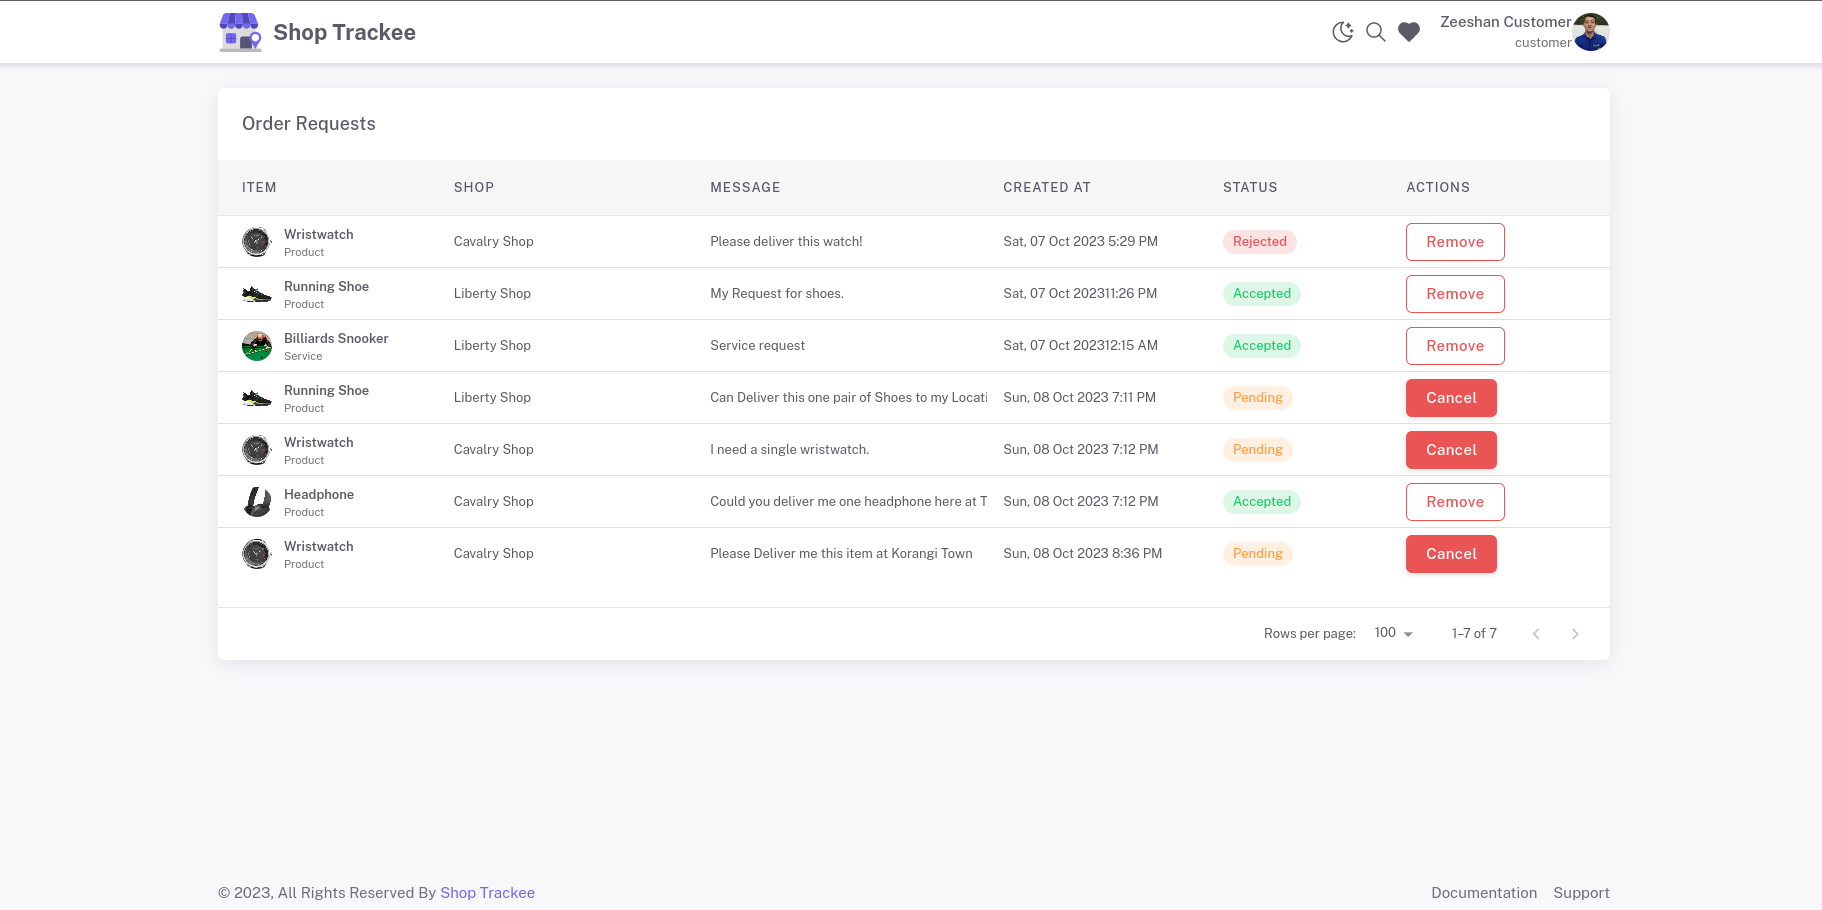
\includegraphics[width=1\textwidth]{customer-order-requests-page}
	\caption{Shop Trackee - Customer Order Requests History}
\end{figure}

\begin{figure}[h]
	\subsection{Customer Favorites}
	\centering
	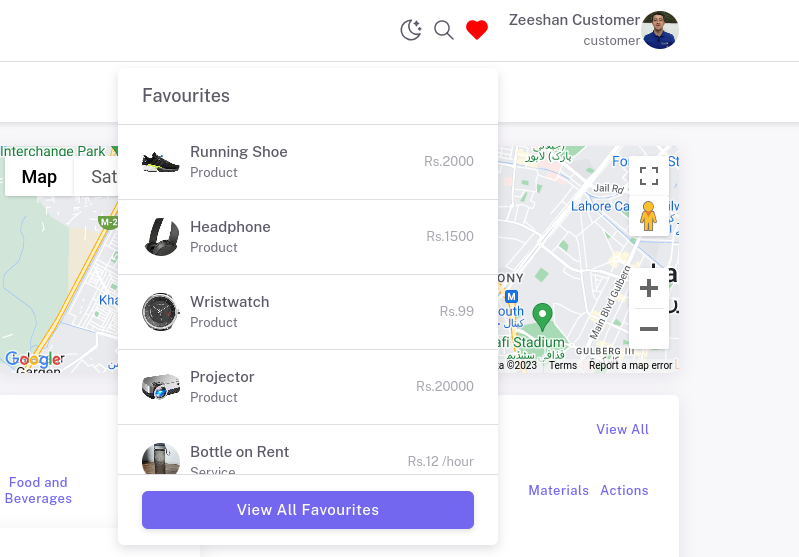
\includegraphics[width=0.8\textwidth]{customer-home-favorites-page}
	\caption{Shop Trackee - Customer Favorites}
\end{figure}
\pagebreak
\begin{figure}[h]
	\subsection{Customer All Favorites}
	\centering
	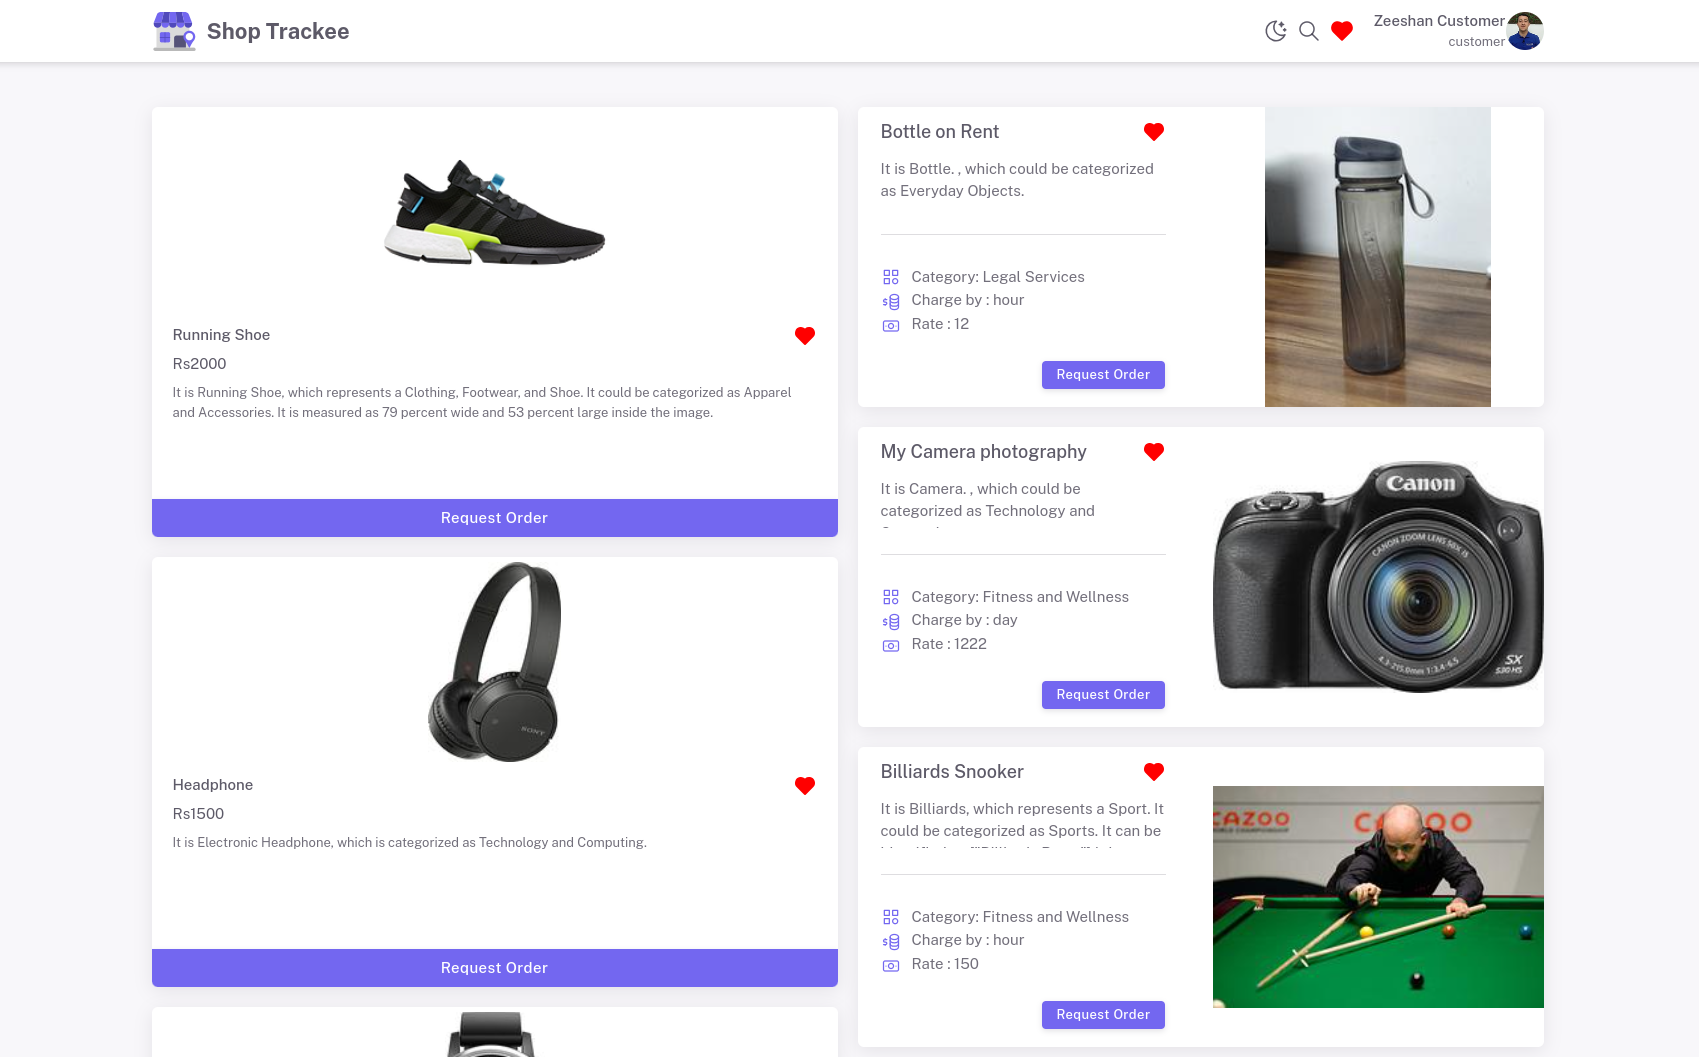
\includegraphics[width=1\textwidth]{customer-all-favorites-page}
	\caption{Shop Trackee - Customer Favorites}
\end{figure}


\begin{figure}[h]
	\subsection{Dark Mode}
	\centering
	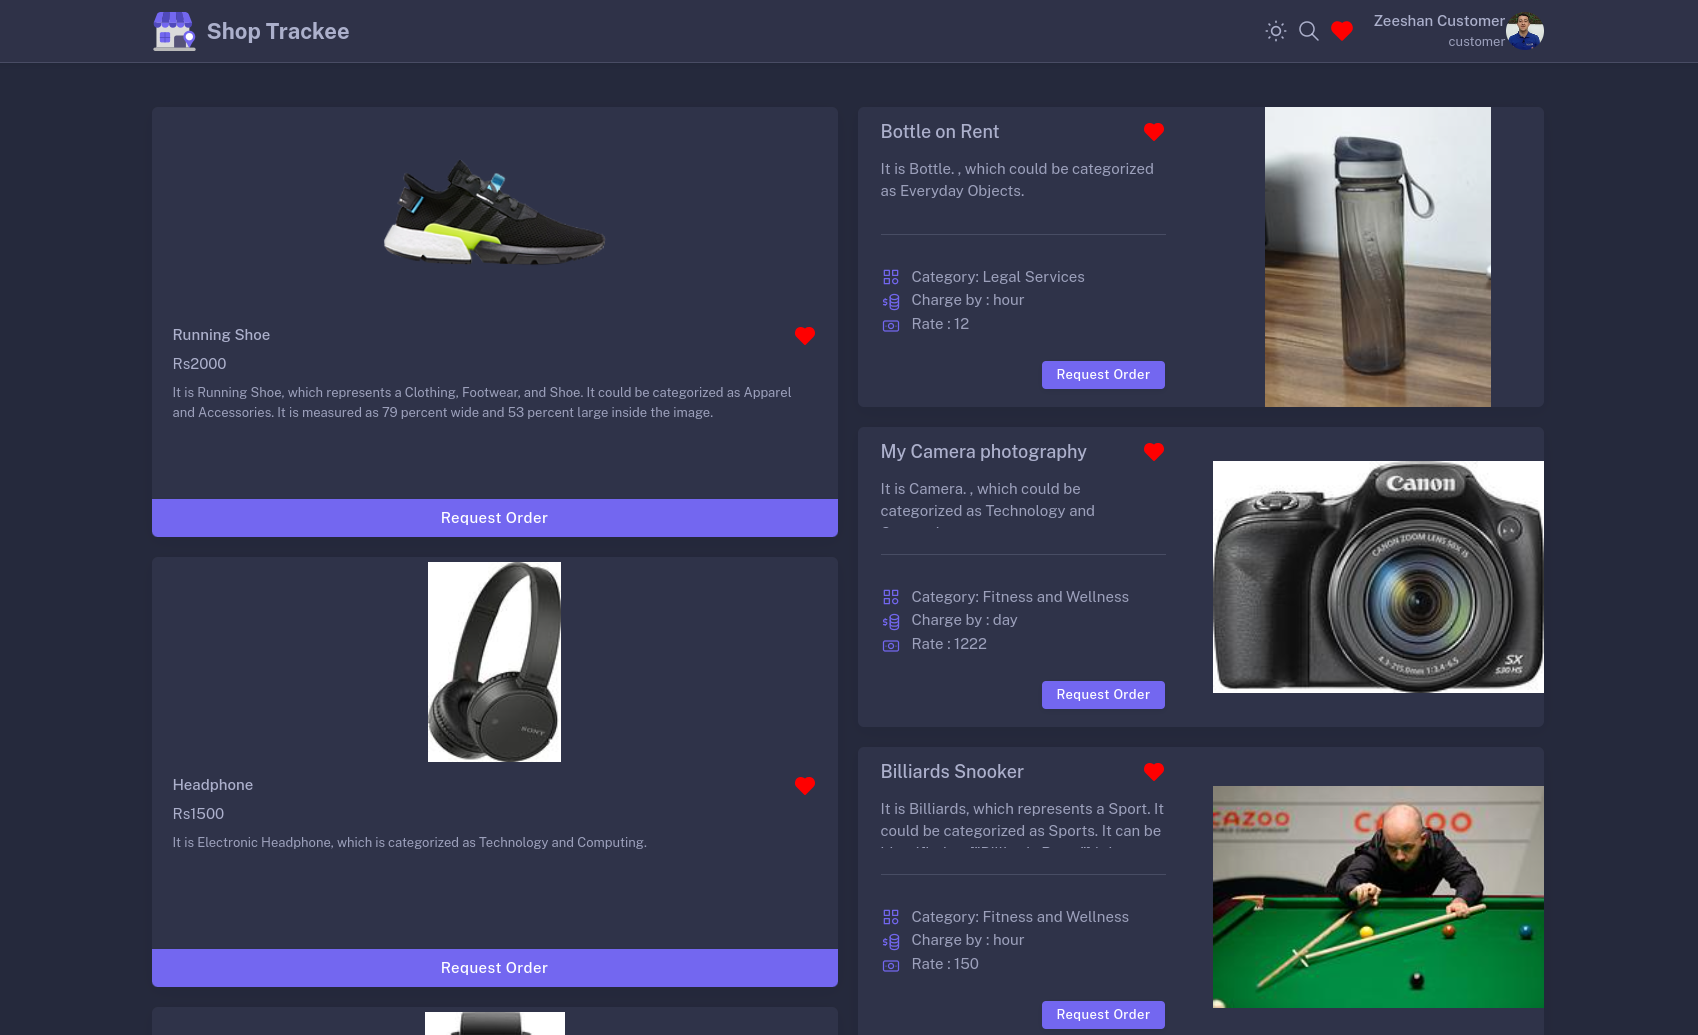
\includegraphics[width=0.9\textwidth]{dark-mode-favorites-page}
	\caption{Shop Trackee - Dark Mode}
\end{figure}

\pagebreak
\section{Hardware Interface}
The "Track My Shop" web application is primarily a software-based system that relies on internet connectivity and web browsers to function. However, there are a few essential hardware components and interfaces that enable its operation:

\begin{itemize}
	\item Computer Systems (Desktops, Laptops, Tablets)
	\item Smartphones and Mobile Devices
	\item Stable Internet Connection
	\item Cameras (for Image Capture)
	\item Global Positioning System (GPS) and Location Services
	\item Input Devices (Keyboards, Mouse, Touchscreens)
\end{itemize}

\subsection{Hardware Requirements}
Here are some minimal requirements of hardware to run this Web Application:
\begin{itemize}
	\item Pentium 4 - 1.9Ghz  
	\item RAM 1 GB+ 
	\item System Storage (minimum 1 GB)
	\item Windows, Linux, Mac, Andriod, IOS
	\item Browsers (Chrome 64+, Edge 79+, Firefox 67+, Opera 51+, Safari 12+)
	\item GPS WGS 84 (World Geodetic System 1984) datum for Google Maps 
\end{itemize}


\section{Evaluation}
Each element of our website is meticulously designed based on the findings of Market Shop Sellers and Customer Research, which takes into account criteria such as technical knowledge, and comprehension.The user is given a seamless experience, allowing them to easily see, update, upload, and manage their data. While designing the website, Human Computer Interaction concepts were taken into account, allowing the user to see where they are presently working and easy to use. Before releasing the website, we make sure that all of the tabs and buttons are visible and double-checked and everything is working properly. Once the website is ready for the user, it will be extensively tested and any necessary changes will be done. Hence the website is user friendly and unambiguous.

\section{Unit Testing}

Unit testing is a crucial component of the development process in "Track My Shop." It involves testing individual units or components of the application to ensure their accuracy, reliability, and correctness. The primary focus is to verify that each unit of the software performs as designed.

In this project, unit testing will encompass the following aspects:

\subsection{Frontend Components} Test individual frontend components like UI elements, input fields, buttons, and their respective functionalities to ensure proper rendering and interactivity.
	
\subsection{Backend API Endpoints} Test the backend API endpoints using testing frameworks to verify their response, data integrity, error handling, and authentication mechanisms.
	
\subsection{Database Interactions} Test the interactions with the database, including CRUD operations, to ensure accurate data retrieval, storage, and manipulation.
	
\subsection{Integration Testing} Conduct integration tests to validate the interaction and communication between different modules, ensuring the overall system functions seamlessly.
	
\subsection{Error Handling and Edge Cases} Perform tests to evaluate the system's behavior under various error conditions and edge cases to guarantee robustness and graceful error handling.


Adopting a comprehensive unit testing strategy will enhance the project's quality, reduce bugs, and provide a stable and reliable application for users.

\section{Test Cases}
Unit testing is a crucial component of the development process in "Track My Shop". It involves testing individual units or components of the application to ensure their accuracy, reliability, and correctness. The primary focus is to verify that each unit of the software performs as designed. Here are some test cases for major units of the application:


\subsection{Frontend Components}

Here are the unit test cases for the frontend components:


% Table for User Registration Form Validation test case
\begin{table}[h]
	\subsubsection{Test Case 1: User Registration Form Validation}
	\centering
	\caption{User Registration Form Validation (TC1)}
	\begin{tabular}{|p{0.3\linewidth}|p{0.6\linewidth}|}
		\hline
		\textbf{Test Case ID} & TC1 \\
		\hline
		\textbf{Test Case Name} & User Registration Form Validation \\
		\hline
		\textbf{Component} & User Registration Form \\
		\hline
		\textbf{Input} & Incomplete or incorrect user registration details \\
		\hline
		\textbf{Expected Output} & Prevent registration and display appropriate validation errors \\
		\hline
		\textbf{Test Steps} & 
		\begin{enumerate}
			\item Fill the registration form with incomplete or incorrect details
			\item Attempt to submit the registration form
			\item Check the interface to verify appropriate validation errors are displayed
		\end{enumerate} \\
		\hline
		\textbf{Execution Result} & Pass \\
		\hline
	\end{tabular}
\end{table}

\pagebreak
% Table for Product Image Uploading test case
\begin{table}[h]
	\subsubsection{Test Case 2: Product/Service Image Uploading \& Recognition}
	\centering
	\caption{Product Image Uploading (TC2)}
	\begin{tabular}{|p{0.3\linewidth}|p{0.6\linewidth}|}
		\hline
		\textbf{Test Case ID} & TC2 \\
		\hline
		\textbf{Test Case Name} & Product/Service Image Uploading and Recognition \\
		\hline
		\textbf{Component} & Product/Service Image Chooser / Image Capturing Camera\\
		\hline
		\textbf{Input} & Image upload/capture request \\
		\hline
		\textbf{Expected Output} & Successful image upload and display in the product/service management UI \\
		\hline
		\textbf{Test Steps} & 
		\begin{enumerate}
			\item Initiate image upload process
			\item Check the Recognize Image button visibility under image
			\item Recognize Image by using button
			\item Check the UI to verify the image is displayed appropriately
			\item Check the product/service form to verify recognized data
		\end{enumerate} \\
		\hline
		\textbf{Execution Result} & Pass \\
		\hline
	\end{tabular}
\end{table}
\pagebreak

\begin{table}[h]
	\subsubsection{Test Case 3: Product/Service Component Rendering}
	\centering
	\caption{Unit Test for Rendering Product/Service Display Component (TC3)}
	\begin{tabular}{|p{0.3\linewidth}|p{0.6\linewidth}|}
		\hline
		\textbf{Test Case ID} & TC3 \\
		\hline
		\textbf{Test Case Name} & Rendering Product/Service Display \\
		\hline
		\textbf{Component} & Product/Service Display Component \\
		\hline
		\textbf{Input} & None (Component rendering) \\
		\hline
		\textbf{Expected Output} & Rendered product/service display \\
		\hline
		\textbf{Test Steps} & \begin{enumerate}
			\item Load the application 
			\item Navigate to the page where the products/services display component is rendered 
		\end{enumerate} \\
		\hline
		\textbf{Execution Result} & Pass \\
		\hline
	\end{tabular}
\end{table}




% Table for Order Request with Message test case
\begin{table}[h]
	\subsubsection{Test Case 4: Order Request with Message}
	\centering
	\caption{Order Request with Message (TC4)}
	\begin{tabular}{|p{0.3\linewidth}|p{0.6\linewidth}|}
		\hline
		\textbf{Test Case ID} & TC4 \\
		\hline
		\textbf{Test Case Name} & Order Request with Message \\
		\hline
		\textbf{Component} & Order Management UI \\
		\hline
		\textbf{Input} & Order request along with an optional message from the customer \\
		\hline
		\textbf{Expected Output} & Successful submission of the order request with the attached message \\
		\hline
		\textbf{Test Steps} & 
		\begin{enumerate}
			\item Select a product and initiate the order request process
			\item Provide additional instructions or messages (optional)
			\item Complete the order request
			\item Check all order requests table to verify the order request was successful
		\end{enumerate} \\
		\hline
		\textbf{Execution Result} & Pass \\
		\hline
	\end{tabular}
\end{table}

\pagebreak
% Table for Search Bar Functionality test case
\begin{table}[h]
	\subsubsection{Test Case 5: Search Box Functionality}
	\centering
	\caption{Search Bar Functionality (TC5)}
	\begin{tabular}{|p{0.3\linewidth}|p{0.6\linewidth}|}
		\hline
		\textbf{Test Case ID} & TC5 \\
		\hline
		\textbf{Test Case Name} & Search Box Functionality \\
		\hline
		\textbf{Component} & Search Bar, Image Capturing Camera, Search Radius Field \\
		\hline
		\textbf{Input} & Search query, Search Image, Distance radius \\
		\hline
		\textbf{Expected Output} & Display of relevant search results \\
		\hline
		\textbf{Test Steps} & 
		\begin{enumerate}
			\item Enter a search query in the search bar
			\item Initiate the search process
			\item Check the interface to verify relevant search results are displayed
		\end{enumerate} \\
		\hline
		\textbf{Execution Result} & Pass \\
		\hline
	\end{tabular}
\end{table}


\subsection{Backend API Endpoints}

Here are the unit test cases for the backend API endpoints:

\begin{table}[h]
	\subsubsection{Test Case 6: Response of Product Listing Endpoint}
	\centering
	\caption{Test Case for Response of Product Listing Endpoint (TC6)}
	\begin{tabular}{|p{0.3\linewidth}|p{0.6\linewidth}|}
		\hline
		\textbf{Test Case ID} & TC6 \\
		\hline
		\textbf{Test Case Name} & Response of Product Listing Endpoint \\
		\hline
		\textbf{Endpoint} & Product Listing \\
		\hline
		\textbf{Input} & Send a request to the product listing endpoint \\
		\hline
		\textbf{Expected Output} & Receive a list of products \\
		\hline
		\textbf{Test Steps} & \begin{enumerate}
			\item Send a valid request to the product listing endpoint 
			\item Receive the response from the endpoint 
		\end{enumerate}\\
		\hline
		\textbf{Execution Result} & Pass \\
		\hline
	\end{tabular}
\end{table}


\begin{table}[h]
	\subsubsection{Test Case 7: Error Handling of Invalid Request}
	\centering
	\caption{Test Case for Error Handling of Invalid Request (TC7)}
	\begin{tabular}{|p{0.3\linewidth}|p{0.6\linewidth}|}
		\hline
		\textbf{Test Case ID} & TC7 \\
		\hline
		\textbf{Test Case Name} & Error Handling of Invalid Request \\
		\hline
		\textbf{Endpoint} & Any API Endpoint \\
		\hline
		\textbf{Input} & Send an invalid request \\
		\hline
		\textbf{Expected Output} & Receive an appropriate error response \\
		\hline
		\textbf{Test Steps} & \begin{enumerate}
			\item Send an invalid request to the specified endpoint
			\item Receive the error response from the endpoint
		\end{enumerate} \\
		\hline
		\textbf{Execution Result} & Pass \\
		\hline
	\end{tabular}
\end{table}


\pagebreak
\subsection{Database Interactions}

% Table for Product Data Retrieval test case
\begin{table}[h]
	\subsubsection{Test Case 8: Product Data Retrieval}
	\centering
	\caption{Product Data Retrieval (TC8)}
	\begin{tabular}{|p{0.3\linewidth}|p{0.6\linewidth}|}
		\hline
		\textbf{Test Case ID} & TC8 \\
		\hline
		\textbf{Test Case Name} & Product Data Retrieval \\
		\hline
		\textbf{Component} & Database Interaction \\
		\hline
		\textbf{Input} & Request to retrieve product data \\
		\hline
		\textbf{Expected Output} & Valid product data from the database \\
		\hline
		\textbf{Test Steps} & \begin{enumerate}
			\item Send a request to retrieve product data	
			\item Check the received product data
		\end{enumerate}\\
		\hline
		\textbf{Execution Result} & Pass \\
		\hline
	\end{tabular}
\end{table}


% Table for Adding New Product test case
\begin{table}[h]
	\subsubsection{Test Case 9: Adding New Product}
	\centering
	\caption{Adding New Product (TC9)}
	\begin{tabular}{|p{0.3\linewidth}|p{0.6\linewidth}|}
		\hline
		\textbf{Test Case ID} & TC9 \\
		\hline
		\textbf{Test Case Name} & Adding New Product \\
		\hline
		\textbf{Component} & Database Interaction \\
		\hline
		\textbf{Input} & New product details (name, description, price, etc.) \\
		\hline
		\textbf{Expected Output} & Product added successfully in the database \\
		\hline
		\textbf{Test Steps} & \begin{enumerate}
			\item Provide input for a new product 
			\item Initiate the process to add the product
			\item Check the response to verify successful addition
			\end{enumerate} \\
		\hline
		\textbf{Execution Result} & Pass \\
		\hline
	\end{tabular}
\end{table}

\pagebreak
\subsection{Integration Testing}

% Table for Integration of User Authentication test case
\begin{table}[h]
	\subsubsection{Test Case 10: Integration of User Authentication}
	\centering
	\caption{Integration of User Authentication (TC10)}
	\begin{tabular}{|p{0.3\linewidth}|p{0.6\linewidth}|}
		\hline
		\textbf{Test Case ID} & TC10 \\
		\hline
		\textbf{Test Case Name} & Integration of User Authentication \\
		\hline
		\textbf{Components} & Authentication Module, Database Interaction \\
		\hline
		\textbf{Input} & User credentials \\
		\hline
		\textbf{Expected Output} & Successful user authentication \\
		\hline
		\textbf{Test Steps} & 
		\begin{enumerate}
			\item Provide user credentials
			\item Initiate the authentication process
			\item Check the response to verify successful authentication
		\end{enumerate} \\
		\hline
		\textbf{Execution Result} & Pass \\
		\hline
	\end{tabular}
\end{table}

% Table for Integration of Product Listing test case
\begin{table}[h]
	\subsubsection{Test Case 11: Integration of Product Listing}
	\centering
	\caption{Integration of Product Listing (TC11)}
	\begin{tabular}{|p{0.3\linewidth}|p{0.6\linewidth}|}
		\hline
		\textbf{Test Case ID} & TC11 \\
		\hline
		\textbf{Test Case Name} & Integration of Product Listing \\
		\hline
		\textbf{Components} & Product Listing Module, Database Interaction \\
		\hline
		\textbf{Input} & Request to list products \\
		\hline
		\textbf{Expected Output} & Successful retrieval of product listing \\
		\hline
		\textbf{Test Steps} & 
		\begin{enumerate}
			\item Send a request to list products
			\item Check the response to verify the successful retrieval of product listing
		\end{enumerate} \\
		\hline
		\textbf{Execution Result} & Pass \\
		\hline
	\end{tabular}
\end{table}

\pagebreak
\subsection{Error Handling and Edge Cases}


% Table for Invalid User Authentication test case
\begin{table}[h]
	\subsubsection{Test Case 12: Invalid User Authentication}
	\centering
	\caption{Invalid User Authentication (TC12)}
	\begin{tabular}{|p{0.3\linewidth}|p{0.6\linewidth}|}
		\hline
		\textbf{Test Case ID} & TC12 \\
		\hline
		\textbf{Test Case Name} & Invalid User Authentication \\
		\hline
		\textbf{Components} & Authentication Module, Database Interaction \\
		\hline
		\textbf{Input} & Incorrect user credentials \\
		\hline
		\textbf{Expected Output} & Authentication failure with appropriate error message \\
		\hline
		\textbf{Test Steps} & 
		\begin{enumerate}
			\item Provide incorrect user credentials
			\item Initiate the authentication process
			\item Check the response to verify authentication failure and error message
		\end{enumerate} \\
		\hline
		\textbf{Execution Result} & Pass \\
		\hline
	\end{tabular}
\end{table}

% Table for Product Listing Empty test case
\begin{table}[h]
	\subsubsection{Test Case 13: Product Listing Empty}
	\centering
	\caption{Product Listing Empty (TC13)}
	\begin{tabular}{|p{0.3\linewidth}|p{0.6\linewidth}|}
		\hline
		\textbf{Test Case ID} & TC13 \\
		\hline
		\textbf{Test Case Name} & Product Listing Empty \\
		\hline
		\textbf{Components} & Product Listing Module, Database Interaction \\
		\hline
		\textbf{Input} & Request to list products when no products are available \\
		\hline
		\textbf{Expected Output} & Successful retrieval with an empty product list \\
		\hline
		\textbf{Test Steps} & 
		\begin{enumerate}
			\item Send a request to list products
			\item Check the response to verify an empty product list
		\end{enumerate} \\
		\hline
		\textbf{Execution Result} & Pass \\
		\hline
	\end{tabular}
\end{table}

% Add more test cases for Error Handling and Edge Cases as needed
%-----------------------
\pagebreak

% Table for Invalid Product Addition test case
\begin{table}[h]
	\subsubsection{Test Case 14: Invalid Product Addition}
	\centering
	\caption{Invalid Product Addition (TC14)}
	\begin{tabular}{|p{0.3\linewidth}|p{0.6\linewidth}|}
		\hline
		\textbf{Test Case ID} & TC14 \\
		\hline
		\textbf{Test Case Name} & Invalid Product Addition \\
		\hline
		\textbf{Components} & Product Management Module, Database Interaction \\
		\hline
		\textbf{Input} & Incomplete or incorrect product details \\
		\hline
		\textbf{Expected Output} & Failure to add the product with an appropriate error message \\
		\hline
		\textbf{Test Steps} & 
		\begin{enumerate}
			\item Provide incomplete or incorrect product details
			\item Attempt to add the product
			\item Check the response to verify the error message
		\end{enumerate} \\
		\hline
		\textbf{Execution Result} & Pass \\
		\hline
	\end{tabular}
\end{table}



%---------------------------------


\pagebreak
\section{Functional Testing}

Functional testing is a critical aspect of ensuring the "Track My Shop" application meets its intended functional requirements. This type of testing involves validating the software's functions and features against the specified requirements and design. It primarily focuses on what the system does.

Functional testing for this project encompasses the following areas:

\subsection{User Authentication and Authorization} Validate the authentication process to ensure users can securely create accounts, log in, and access appropriate functionalities based on their roles.

\subsection{Product and Service Listings} Verify that sellers can effectively list their products and services using various methods, including image recognition and manual entry, and customers can view and search these listings.

\subsection{Order Placement and Management} Test the ordering process to ensure customers can place orders for products and services, sellers receive order requests, and they can manage and respond to these orders appropriately.

\subsection{Location-Based Features} Validate the location-based functionalities such as finding nearby shops, setting a search radius, and accessing directions to physical shops.

\subsection{Search and Filtering} Verify the accuracy and efficiency of the search and filtering capabilities, allowing users to search for products, services, or shops based on various criteria.

\subsection{Error Handling} Test the system's behavior under erroneous conditions, ensuring that appropriate error messages and notifications are displayed to users.

\subsection{UI/UX Testing} Evaluate the user interface and overall user experience to ensure it is intuitive, consistent, and adheres to design guidelines.
	

Functional testing ensures that the "Track My Shop" application performs its intended functions correctly, providing users with a seamless and reliable experience.


\subsection{Testing Requirements}

Functional testing for this web application necessitates a comprehensive approach that covers various functionalities and ensures their correctness and reliability. The testing requirements include:

\subsubsection{User Authentication:}
	\begin{itemize}
		\item Verify that users can create accounts securely with the necessary role and personal information.
		\item Test login functionality, ensuring users can authenticate themselves with correct credentials.
		\item Validate the behavior of the system in case of incorrect login attempts, including appropriate error messages.
	\end{itemize}
	
\subsubsection{Product and Service Listings:}
	\begin{itemize}
		\item Ensure sellers can accurately list products and services using various methods like image recognition, capturing image, and choosing image manually or manual entry.
		\item Validate that sellers can edit, delete, and update product and service information as needed.
		\item Verify that customers can view and filter product and service listings with ease.
	\end{itemize}
	
\subsubsection{Orders Management:}
	\begin{itemize}
		\item Test the process of requesting orders, ensuring customers can successfully initiate orders for desired products and services.
		\item Validate that sellers receive order requests promptly and can manage them effectively, including accepting or rejecting order requests.
		\item Verify that customers receive timely notifications and updates on their orders.
	\end{itemize}
	
\subsubsection{Location-Based Features:}
	\begin{itemize}
		\item Ensure users can find nearby shops based on their location and specified search radius.
		\item Validate the accuracy of location-based search results, providing users with relevant and nearby options.
		\item Test the functionality of accessing directions to physical shops from the user's current location.
	\end{itemize}
	
\subsubsection{Search and Filtering:}
	\begin{itemize}
		\item Validate the accuracy and efficiency of the search feature, allowing users to search for products, services, or shops based on keywords.
		\item Test capabilities to ensure users can search based on image, categories, or other relevant criteria.
	\end{itemize}
	
\subsubsection{Error Handling:}
	\begin{itemize}
		\item Verify that the system displays appropriate error messages and notifications for incorrect inputs or erroneous actions.
		\item Test the behavior of the system under unexpected conditions, ensuring graceful handling of errors to prevent system crashes.
	\end{itemize}
	
\subsubsection{UI/UX Testing:}
	\begin{itemize}
		\item Validate that the user interface is consistent, intuitive, and adheres to design guidelines.
		\item Test the responsiveness of the application across various devices and screen sizes.
	\end{itemize}

These testing requirements form the basis for comprehensive functional testing, ensuring the application meets its intended functionalities reliably and accurately.












% Chapter 5

\chapter{Conclusion \& Future Work} % Main chapter title

\label{Chapter5} % For referencing the chapter elsewhere, use \ref{Chapter1}

\lhead{Chapter 5. \emph{Conclusion \& Future Work}} % This is for the header on each page - perhaps a shortened title

%----------------------------------------------------------------------------------------

\section{Conclusion}
The "Track A Shop: Web App" project introduces a user-friendly and affordable web application tailored for small businesses and local service providers. By offering a centralized platform accessible through standard web browsers on various devices, the project enables businesses to showcase their products and services online. Leveraging image recognition and geolocation features, the application simplifies the process of product listing and enhances the search experience for customers.

The main focus of the project has been to make digitalization affordable and accessible for small businesses. Through a well-structured codebase and an intuitive user interface, the application ensures a seamless and engaging experience for both sellers and customers. The use of modern technologies like Next.js, Ruby on Rails, AWS, and PostgreSQL ensures the application is robust and scalable.

Moving forward, gathering user feedback and staying updated with evolving technologies will be key to refining and improving the application. "Track A Shop: Web App" strives to contribute to a more connected digital economy, facilitating a stronger bond between local businesses and their communities.


\section{Future Work}
In the following, we outline the potential areas for future work and enhancements to further improve the "Track A Shop: Web App" platform.

\subsection{Enhanced User Experience:}

Conduct usability testing and gather extensive user feedback to refine the user interface, making it even more intuitive and appealing to a broader user base.

\subsection{Machine Learning Integration:}

Explore the integration of machine learning algorithms to enhance the image recognition capabilities, allowing for more accurate and efficient product and service identification from uploaded images.

\subsection{Facial Recognition}
Investigate the possibility of integrating facial recognition technology for profile data completion using profile image and enhanced security within the application.

\subsection{Personalized Recommendations:}

Implement recommendation algorithms based on user preferences and behavior, offering personalized product and service recommendations to customers, thereby enhancing user engagement and sales.

\subsection{Integration of Payment Gateways:}

Incorporate secure and widely used payment gateways to facilitate online transactions directly within the application, streamlining the purchase process for customers.

\subsection{Multi-Language Support:}

Introduce multi-language support to make the application accessible to a more diverse audience, promoting inclusivity and user engagement across different regions and languages.

\subsection{Real-Time Chat and Customer Support:}

Integrate a real-time chat feature to enable direct communication between customers and sellers, fostering better customer support and trust.

\subsection{Inventory Management System:}

Develop an integrated inventory management system for sellers to efficiently track, manage, and update their product and service offerings in real-time.

\subsection{Social Media Integration:}

Integrate social media sharing functionalities to enable users to easily share their favorite products and services with their social network, enhancing the application's reach and user engagement.

\subsection{Third Party Integration for Sign-in:}

Integrate popular third-party authentication services (e.g., Google (for Google My Business), Facebook, Instagram etc.) to allow users to sign in using their existing credentials, enhancing user onboarding and convenience.

\subsection{Integration with Other E-commerce Platforms:}

Investigate the potential for integrating with established e-commerce platforms to allow seamless synchronization of product listings and sales, potentially broadening the reach and opportunities for sellers.

\subsection{Customer Analytics Dashboard:}

Create a comprehensive analytics dashboard for sellers, providing insights into customer behavior, purchase patterns, and popular products, aiding in informed business decisions.

\subsection{Mobile Application Development:}

Extend the project by developing dedicated mobile applications (iOS and Android) to cater to the increasing number of users accessing the platform via mobile devices.

\subsection{Offline Access and Progressive Web App (PWA):}

Implement Progressive Web App features to ensure limited functionality and access to the application even in offline mode, enhancing user experience.

\subsection{Import data from Business Websites:}

Explore features that allow sellers to import or list their existing products or services from already established business websites, streamlining the onboarding process and saving time for sellers.

\subsection{Integration with Local Services:}

Collaborate with local delivery services to enable seamless integration for order deliveries, further enhancing convenience for customers and boosting sales for sellers.
These future directions offer a glimpse into the potential growth and evolution of the "Track A Shop: Web App" project, ensuring its continual adaptation to emerging technologies and the evolving needs of both businesses and consumers in the dynamic digital landscape.




\backmatter

%----------------------------------------------------------------------------------------
%	BIBLIOGRAPHY
%----------------------------------------------------------------------------------------
\label{References}


\end{document}
